\documentclass[english,11pt]{article}

\pdfoutput=1

\usepackage[T1]{fontenc}
\usepackage[latin9]{inputenc}
\usepackage{verbatim}
\usepackage{float}
\usepackage{amsthm}
\usepackage{amsmath}
\usepackage{amssymb}
\usepackage{graphicx}
%\usepackage{multirow}
\usepackage{color}
\usepackage{url}
\usepackage{caption}
\usepackage{subcaption}
\usepackage{mathtools} 
\usepackage[margin=1.2in]{geometry}


\newcommand{\LL}{\mathcal{L}}
\newcommand{\E}{\mathbb{E}}
\newcommand{\I}{\mathcal{I}}
\newcommand{\ep}{\varepsilon}
\newcommand{\Z}{\mathbb{Z}}
\newcommand{\GCD}{\mathbf{GCD}}
\newcommand{\XX}{\mathcal{X}}
\newcommand{\SUM}{\text{sum}}
\newcommand{\1}{\mathbf{1}}


\newcommand{\TODO}[1]{{\color{red}{[#1]}}}

\makeatletter

%%%%%%%%%%%%%%%%%%%%%%%%%%%%%% Textclass specific LaTeX commands.
\numberwithin{equation}{section}
%\numberwithin{figure}{section}
\theoremstyle{plain}
\newtheorem{thm}{\protect\theoremname}[section]
\theoremstyle{definition}
\newtheorem{defn}[thm]{\protect\definitionname}
\theoremstyle{remark}
\newtheorem{claim}[thm]{\protect\claimname}
\theoremstyle{plain}
\newtheorem{lem}[thm]{\protect\lemmaname}

\newtheorem*{lem*}{Lemma}

\theoremstyle{remark}
\newtheorem{rem}[thm]{\protect\remarkname}
\theoremstyle{plain}
\newtheorem{corollary}[thm]{\protect\corollaryname}
\theoremstyle{plain}
\newtheorem{proposition}[thm]{\protect\propositionname}
%%%%%%%%%%%%%%%%%%%%%%%%%%%%%% User specified LaTeX commands.
%\usepackage{slashbox}

\usepackage{babel}
\providecommand{\claimname}{Claim}
\providecommand{\definitionname}{Definition}
\providecommand{\lemmaname}{Lemma}
\providecommand{\remarkname}{Remark}
\providecommand{\theoremname}{Theorem}
\providecommand{\corollaryname}{Corollary}
\providecommand{\propositionname}{Proposition}


\newcommand{\reals}{\mathbb{R}}
\newcommand{\RL}{\mathbb{R}^L}
\newcommand{\CL}{\mathbb{C}^L}
\newcommand{\RN}{\mathbb{R}^N}
\newcommand{\RNN}{\mathbb{R}^{N\times N}}
\newcommand{\CNN}{\mathbb{C}^{N\times N}}
\newcommand{\inner}[1]{\left\langle {#1} \right\rangle}
\newcommand{\hx}{\hat{x}} 
\newcommand{\one}{\mathbf{1}} 
\newcommand{\SNR}{\ensuremath{\textsf{SNR}}}

\begin{document}

\title{Toward single particle reconstruction without particle picking: Breaking the detection limit}


\author{Tamir Bendory, Nicolas Boumal, William Leeb and Amit Singer}
\maketitle

\begin{abstract}
	Here comes the abstract
\end{abstract}

\section{Introduction}

\TODO{Revise--Cryo--electron microscopy (cryo--EM) is an innovative technology for single particle reconstruction (SPR) of macromolecules.} 
%In recent years, structures of many molecules, previously regarded as insurmountable, are now being reconstructed to near-atomic resolution
%; see for instance~\cite{kuhlbrandt2014resolution,bartesaghi20152,smith2014beyond}.
%This technological advancement was recognized by the 2017 Nobel Prize in Chemistry~\cite{nobel}. 
% 
In a cryo--EM experiment, biological samples are rapidly frozen in a thin layer of vitreous ice. Within the ice, the molecules are randomly oriented and positioned. The microscope produces a 2-D image of the samples embedded in the ice called a \emph{micrograph}. Each micrograph contains tomographic projections of the samples at unknown locations and under unknown viewing directions. The goal is to construct 3-D models of the molecules from the micrographs.

The signal to noise ratio ($\SNR$) of the projections in the micrographs is a function of two dominating factors. On the one hand, the $\SNR$ is a function of the electron dose. To keep radiation damage within acceptable bounds, the dose must be kept low, which leads to high noise levels. On the other hand, the $\SNR$ is a function of the molecule size. The smaller the molecules, the fewer detected electrons carry information about them.

%\paragraph{Particle picking.}
All contemporary methods in the field split the reconstruction procedure in several stages.
The first stage consists in extracting the various particle projections from the micrographs. This is called \emph{particle picking}. Later stages aim to construct a 3-D model of the molecule from these projections. The quality of the reconstruction eventually hinges on the quality of the particle picking stage. As can be seen from Figure~\ref{fig:micro_example}, locating the particles becomes increasingly challenging as the $\SNR$ degrades.

Crucially, it can be shown that reliable detection of individual particles is impossible below a certain critical $\SNR$. This fact has been recognized early on by the cryo-EM community. In particular, in a highly cited paper from 1995, Henderson~\cite{henderson1995limitations} investigates the following questions:
\begin{quote}
	\emph{For the purposes of this review, I would like to ask the question: what is the smallest size of free-standing molecule whose structure can in principle be determined by phase-contrast electron microscopy? Given what has already been demonstrated in published work, this reduces to the question: what is the smallest size of molecule for which it is possible to determine from images of unstained molecules the five parameters needed to define accurately its orientation (three parameters) and position (two parameters) so that averaging can be performed?}
\end{quote}
In that paper and in others that followed (e.g.,~\cite{glaeser1999electron}), it was established that particle picking is impossible for molecules below a certain weight.
%This has often been understood as meaning that particle reconstruction itself is impossible for such molecules~\cite{khoshouei2017cryo,liu2018nearatomic,liang2017phase}. \TODO{This list may be unfair, as some of these papers (in particular, \cite{liang2017phase}) just state that small molecules are very challenging, which is true.}
As a result, it is impossible to reconstruct such small molecules by any of the existing computational pipelines for single particle analysis, as the particles themselves cannot be picked from the micrographs.
%
%\TODO{either here, or in a close neighborhood of this paragraph you should mention the advances that the field has made in recent years towards reconstruction of small size molecules: mention Volta phase plate and the scaffolding cage (and cite the papers I sent you).}
This has motivated recent technical advances in the field, including the use of Volta phase plates~\cite{khoshouei2017cryo,liang2017phase} and scaffolding cages~\cite{liu2018nearatomic}.
%
%
Despite this progress, detecting small molecules (below 50 kDa) in the micrographs remains a challenge.
We note that nuclear magnetic resonance (NMR) spectroscopy and X-ray crystallography are well suited to reconstruct small molecules. Yet, cryo--EM has a lot to offer even for molecules with already known structures obtained via NMR spectroscopy or X-ray crystallography, because these methods have limited ability to distinguish conformational variability. \TODO{Need a ref for this claim.}

In this paper, we argue that there is a gap between the two questions in the quoted excerpt above, and that one may be able to exploit it to design better reconstruction algorithms.
Specifically, the impossibility of particle picking does not necessarily imply impossibility of particle reconstruction.
%This can be understood from a statistical point of view by counting the number of parameters that one aims to estimate. \TODO{For a given target resolution, the number of parameters required to describe the 3-D model of the molecule is fixed: it does not depend on the amount of data collected. In contrast, particle picking involves estimation of several so-called nuisance parameters for each projection present in the micrographs, such as their locations for example. To overcome low $\SNR$s, the ratio of data to parameters must increase. This is impossible if the number of parameters grows with the amount of data collected, but not so if the number of parameters remains fixed. Simply put, the key is to bypass the particle picking stage.}
%%Thus, acquiring more data does not necessarily allow to improve the particle picking stage, whereas it should in principle allow to improve the molecule reconstruction.
%%Indeed, the signal itself (the many different views of the molecule) is still present in the micrograph: 
%Indeed, in principle at least, the micrograph does contain the necessary information (several views of the molecule(s) of interest). While we may not be able to locate these views, we may still be able to extract the relevant information through other means.
Indeed, the aim is only to reconstruct the molecule: estimating the locations of the particles in the micrograph is merely a helpful intermediate stage when it can be done. Our main message is that the limits particle picking imposes on molecule size do not translate into limits on particle reconstruction.

%\TODO{Paragraph about the simplified model}
As a proof of concept, we study a simplified model where an unknown image appears numerous times at unknown locations in several micrographs, each affected by additive Gaussian noise---see Figure~\ref{fig:micro_example} for an illustration.
The goal is to estimate the planted image. The task is interesting in particular when the $\SNR$ is low enough that particle picking cannot be done reliably.
%Figure~\ref{fig:Einst_example} displays the results of our method, detailed in Section~\ref{sec:results}.
A precise mathematical formulation of the model, including an extension where more than one planted images are to be recovered, is provided in Section~\ref{sec:methods}.
To be clear, we do not consider here many prominent features of real SPR experiments and do not aim to reconstruct any 3-D structure. Instead, we solve a simpler problem that we believe captures key elements of the SPR problem. We note that similar models emerge in spike sorting~\cite{lewicki1998review}, passive radar~\cite{gogineni2017passive} and system identification~\cite{ljung1998system}.

In order to recover the planted image, we use autocorrelation analysis. In a nutshell, we relate the autocorrelation functions of the micrographs to the autocorrelation functions of the planted image.
%To do so, we assume the image occurrences are well separated.
For any noise level, these autocorrelations can be estimated to any desired accuracy, provided individual occurrences of the image are well separated and the image appears sufficiently many times in the micrographs. Importantly, there is no need to detect individual occurrences. The autocorrelations of the micrographs are straightforward to compute and require only one pass over the data. These directly yield estimates for the autocorrelations of the image. To estimate the image itself from its estimated autocorrelations, we solve a nonlinear inverse problem via least-squares or a phase retrieval algorithm; see Figure~\ref{fig:Einst_example} for an illustration and Section~\ref{sec:methods} for details. As a side note, we mention that expectation-maximization (EM)---a popular framework in SPR---is intractable for this problem; see Appendix~\ref{sec:theory} for a discussion.

Another interesting feature of the described approach pertains to model bias, whose importance in cryo-EM was stressed by a number of authors~\cite{vanheel1992correlation,shatsky2009method,henderson2013avoiding,vanheel2013finding}. In the classical ``Einstein from noise'' experiment, multiple realizations of pure noise are aligned to a picture of Einstein using cross-correlation and then averaged. In~\cite{shatsky2009method}, it was shown that the averaged noise rapidly becomes remarkably similar to the Einstein template. In the context of cryo--EM, this experiment exemplifies how prior assumptions about the particles may influence the reconstructed structure. This model bias is common to all particle picking methods based on template matching. In our approach, no templates are required, thus significantly reducing concerns about model bias.


%\TODO{Paragraph about bias; can also mention computational aspects (single pass, etc.)}

%\TODO{Already mention challenges? I think it's a good place.} -- no, not here: in conclusion

%\clearpage



%\begin{figure}[h!]
%	\centering
%	\begin{subfigure}[h]{0.3\textwidth}
%		\centering
%		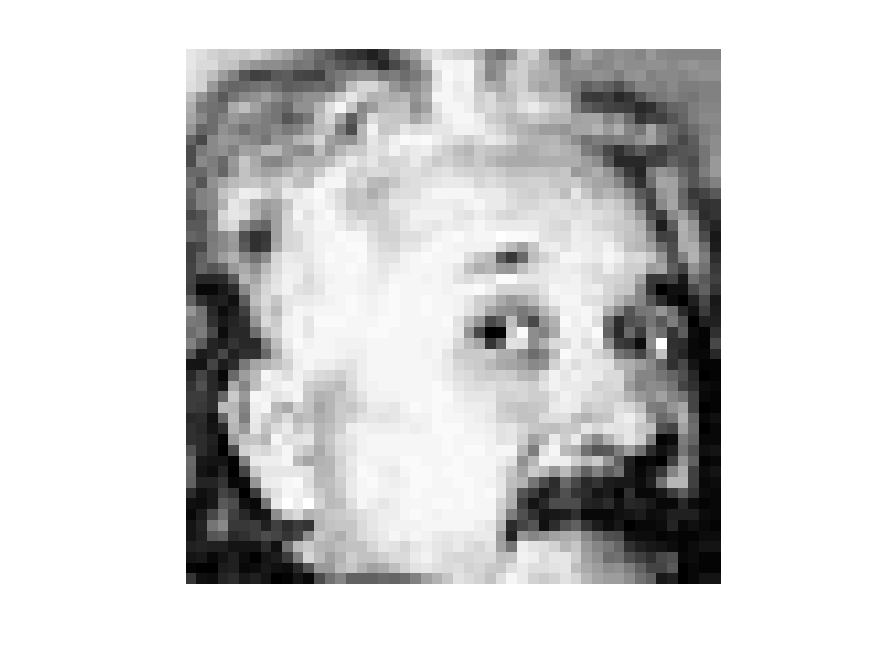
\includegraphics[scale=0.3]{Einstein}
%		\caption{\label{fig:Einstein}Einstein image (template)}
%	\end{subfigure}%
%	\begin{subfigure}[h]{0.3\textwidth}
%		\centering
%		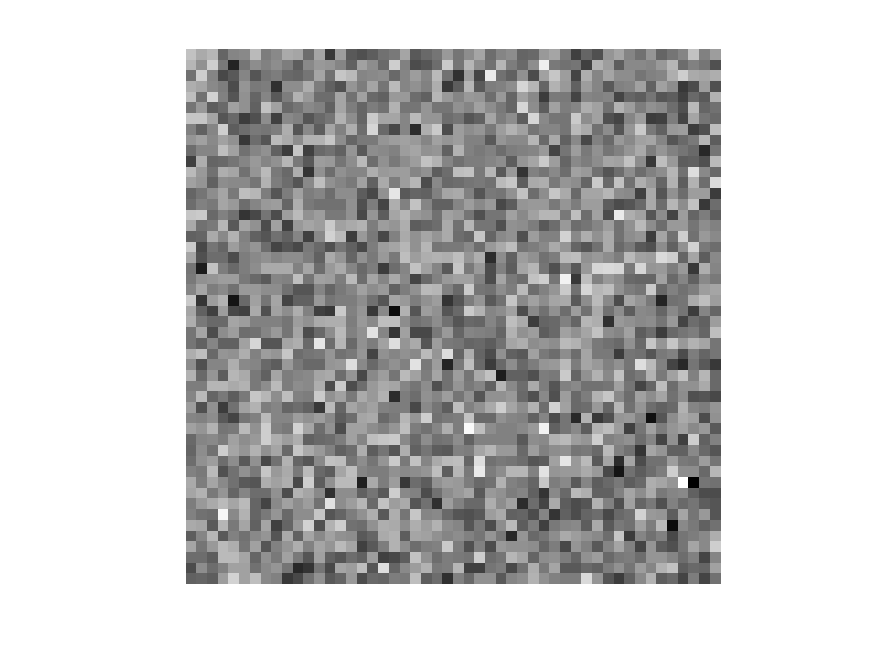
\includegraphics[scale=0.3]{Einstein_from_noise_n10}
%		\caption{$n = 10$}
%	\end{subfigure}
%	\begin{subfigure}[h]{0.3\textwidth}
%		\centering
%		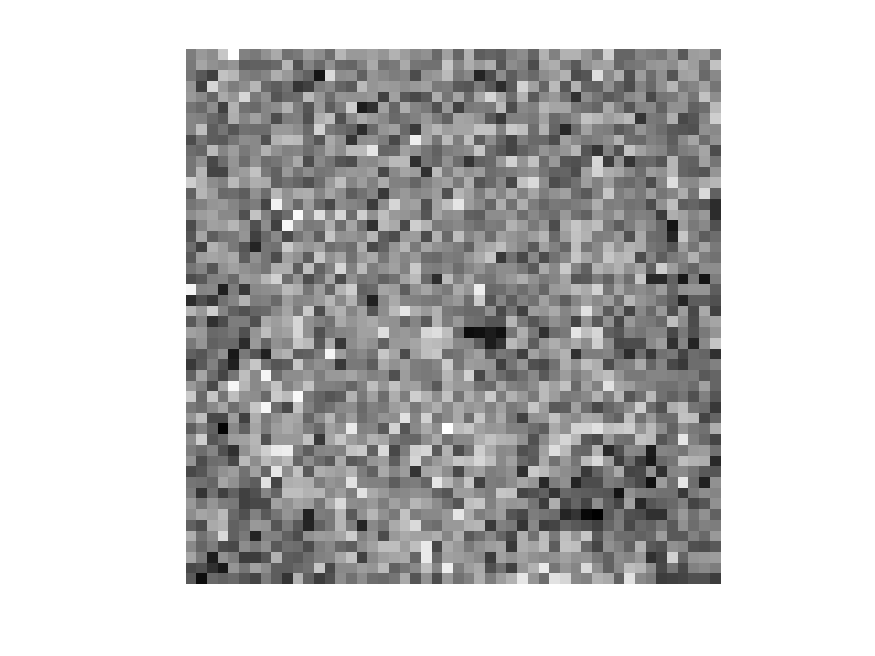
\includegraphics[scale=0.3]{Einstein_from_noise_n100}
%		\caption{$n = 10^2$}
%	\end{subfigure}

%	\begin{subfigure}[h]{0.3\textwidth}
%	\centering
%	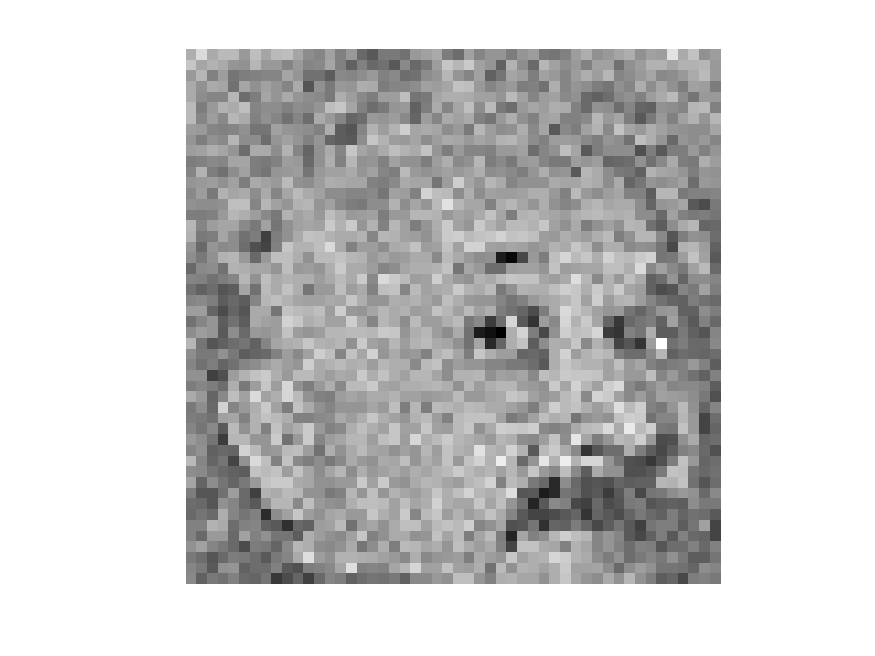
\includegraphics[scale=0.3]{Einstein_from_noise_n1000}
%	\caption{$n = 10^3$}
%\end{subfigure}%
%\begin{subfigure}[h]{0.3\textwidth}
%	\centering
%	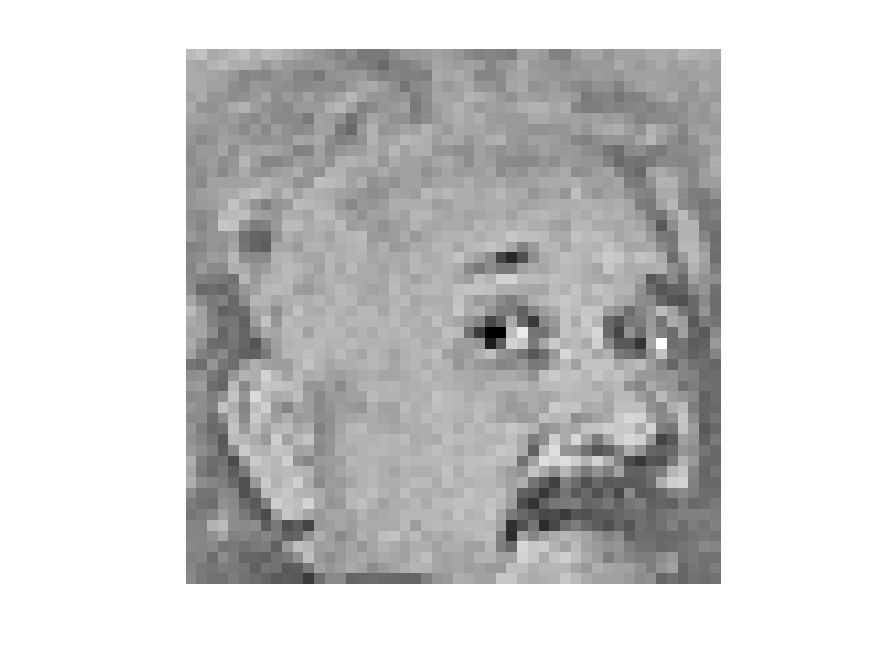
\includegraphics[scale=0.3]{Einstein_from_noise_n10000}
%	\caption{$n = 10^4$}
%\end{subfigure}
%\begin{subfigure}[h]{0.3\textwidth}
%	\centering
%	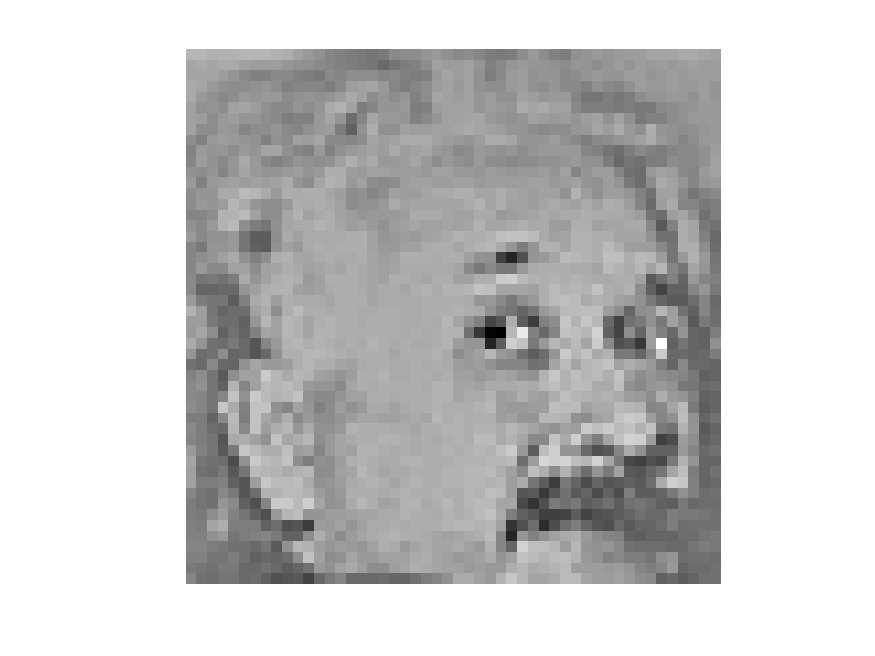
\includegraphics[scale=0.3]{Einstein_from_noise_n100000}
%	\caption{$n = 10^5$}
%\end{subfigure}

%\caption{\label{fig:EinsteinFromNoise} Einstein from noise experiment. As a template, we used Einstein's image of size $50\times 50$ pixels. We drawn $n$ images of the same size whose entries are composed of i.i.d.\ Gaussian entries with the same mean and variance as Einstein's image. Each noise image was aligned with respect to the template by the maximal value of their cross correlation. After the alignment, all the images were averaged. As can be seen, the more pure noise images we use, the closer the averaged image to the template.   }	
%\end{figure}

%Besides the model bias, particle pickers have several limitations due to the high noise level, in particular for small particles and in low contrast. 
%As a result, the projections in the 2-D images are typically not centered; including the correct centers as parameters dramatically increases the complexity of reconstruction algorithms.
%In addition, the information from particles that are too close to each other is usually neglected. Hence, valuable information that can be harnessed is omitted. 

%\paragraph{Simplified model for SPR}

%In this paper, we present a preliminary study that aims to show that estimating a particle 
%directly from the micrograph, without identifying the location of individual particle images in the micrograph, might be possible. 

%In particular, we consider the toy problem of estimating a set of signals $x_1,\ldots,x_K$ from their multiple occurrences in unknown  locations in a noisy data sequence $y$. Here, $y$ plays the role of the micrograph and the $K$ signals can be thought of as $K$ different viewing directions of the particle, each of which  appears multiple times in the micrograph. 
%A precise mathematical formulation of the model and the estimation problem is provided in Section~\ref{sec:methods}.
%To be clear, we do not consider here many prominent features of real SPR experiments and do not aim to reconstruct any 3-D structure; instead, we solve a simpler problem that we believe captures key elements of the true SPR problem. We also mention in passing that similar models emerge in different scientific fields, such as spike sorting~\cite{lewicki1998review}, passive radar~\cite{gogineni2017passive} and system identification~\cite{ljung1998system}.

\begin{figure}[t]
	\centering
	\begin{subfigure}[h]{0.33\textwidth}
		\centering
		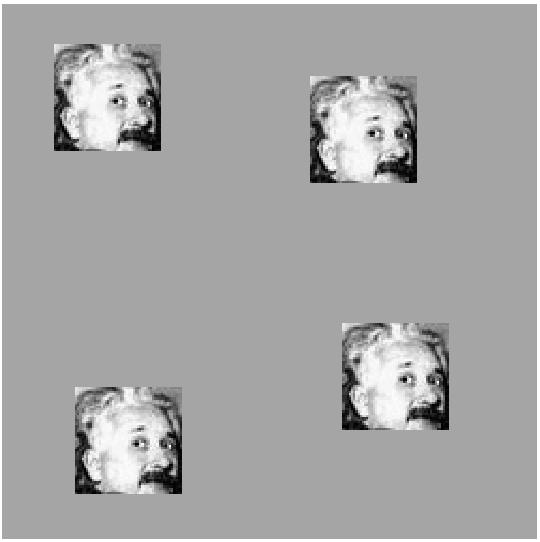
\includegraphics[scale=0.5]{micrograph_Einstein_example_clean}
		\caption{$\sigma = 0$}
	\end{subfigure}%
	\begin{subfigure}[h]{0.33\textwidth}
		\centering
		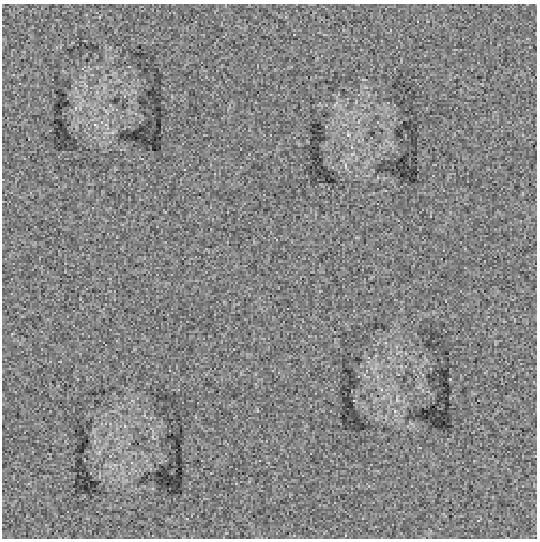
\includegraphics[scale=0.5]{micrograph_Einstein_example_s05}
		\caption{$\sigma = 0.5$}
	\end{subfigure}
	\begin{subfigure}[h]{0.33\textwidth}
		\centering
		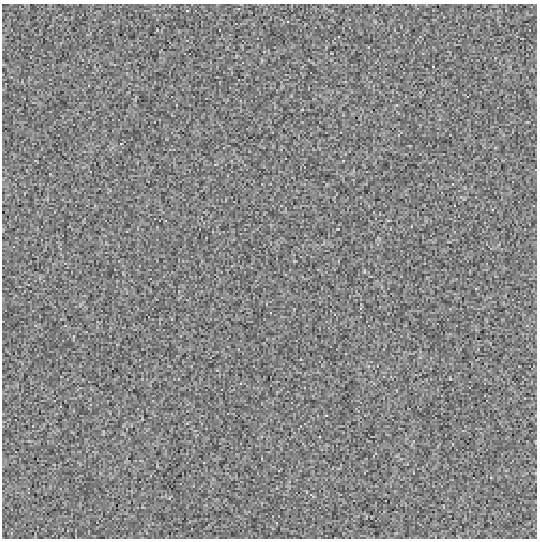
\includegraphics[scale=0.5]{micrograph_Einstein_example_s3}
		\caption{$\sigma = 3$}
	\end{subfigure}
	\caption{\label{fig:micro_example} Example of micrographs of size $250\times 250$ with additive white Gaussian noise of variance $\sigma^2$ for increasing values of $\sigma$. Each micrograph contain the same four occurrences of a $50 \times 50$ image of Einstein. In panel (c), the noise level is such that it is very challenging to locate the occurrences of the planted image. In fact, it can be shown that at low $\SNR$, reliable detection of individual image occurrences is impossible, even if the true image is known. By analogy to cryo-EM, this depicts a scenario where particle picking cannot be done.}	
\end{figure}


%\paragraph{Autocorrelation analysis.}
%We now return to the general problem of estimating $x_1,\dots,x_K$ from the noisy observation $y$.
%In order to recover the signals $x_1,\dots,x_K$ from the data, we use autocorrelation analysis.
%In a nutshell, the method consists of two stages. First, we estimate a mixture (i.e., linear combination) of the low--order autocorrelation functions of the signals from the data. These quantities can be estimated, to any desired accuracy, if individual occurrences are separated by the maximum signal size and each signal appears sufficiently many times in the data. There is no need to detect individual occurrences.
%In the second stage, the signals are estimated from the mixed autocorrelations using a nonconvex least-squares (LS) algorithm or a phase retrieval algorithm; see Section~\ref{sec:methods} for details.
%This method requires only one pass over the data and can recover the signals in any $\SNR$, if the signals appear enough times in the data. As a side note, we mention that expectation-maximization---a popular framework in SPR---is intractable for this problem (see Appendix~\ref{sec:theory}  for more details). 


%\paragraph{Model bias.} The significance of the model bias in cryo--EM was stressed in~\cite{shatsky2009method,henderson2013avoiding} and demonstrated by the ``Einstein from noise'' example.
%In this experiment, the image of Einstein is correlated with multiple images of pure noise. The noisy images are aligned to Einstein's image using cross-correlation and then averaged. 
%In~\cite{shatsky2009method}, it was shown that with merely  1000 noise images, the averaged image is remarkably similar to the template image of Einstein rather than to pure noise.
%In Figure~\ref{fig:EinsteinFromNoise} we conducted this experiment with different number of noise images. With merely 1000 noise images, Einstein's face is clearly observed in the averaged image. With $10,000$  image, the output is remarkably similar to the template image of Einstein rather than to pure noise. Crucially, the more noisy images we use, the more severe the model bias towards the template. 
%In the context of cryo--EM, this example demonstrates how our prior assumptions about the particle may influence the reconstructed structure.
%This true in general to any method which is based on template matching.
%\TODO{Do we have a nice experiment to exemplify the phenomenon?}


\section{Results} \label{sec:results}

%\TODO{Results: What answer was found to the research question; what did the study find? Was the tested hypothesis true?}

%To support the claim that it may be possible to bypass particle picking in SPR from micrographs, as a proof of concept,
We conducted two experiments in the simplified image formation model described in the introduction:
\begin{enumerate}
	\item The first experiment aims to recover a 2-D image from an increasing number of micrographs with high noise, similar to the rightmost panel of Figure~\ref{fig:micro_example}. This is done using moments of second order, as these are sufficient to recover a 2-D image up to elementary symmetries;
	\item The second experiment aims to recover three distinct 1-D signals from an increasing number of 1-D micrographs with high noise. For this task, it is necessary to use moments up to third order.
\end{enumerate}
As outlined below, we find that it is indeed possible to recover good estimates of the ground truth signals from the highly corrupted micrographs, without particle picking. Furthermore, we find that the quality of estimation increases with the amount of data collected, despite the fact that particle picking remains challenging. The methods section provides additional details. In the discussion section, we outline how the general approach could be extended to full 3D SPR.


%In this section we describe  some numerical experiments and show results. The experimental details and the algorithms are discussed at length in Section~\ref{sec:methods}.

In the first experiment, we estimated Einstein's image of size $50\times 50$ and mean zero from a growing number of micrographs, each of size $4096\times 4096$ pixels. A micrograph contains, on average, 700 occurrences of the target image at random locations. The latter are chosen so that two occurrences are always separated by at least 49 pixels. Thus, about 10\% of each micrograph contains signal. The micrographs are contaminated with additive white Gaussian noise with standard deviation $\sigma=3$ (this corresponds to $\SNR=1/20$). This high noise level is illustrated in the right panel of Figure~\ref{fig:micro_example}. In this first experiment, we assume knowledge of $\sigma$ and of the total number of signal occurrences across all micrographs.

We compute the average autocorrelation of the micrographs (equivalently, the average of their power spectra). This is a particularly simple computation. In the methods section, we show how, owing to separation of the occurrences, a determined portion of the averaged autocorrelation allows to estimate the power spectrum of the unknown image itself. Mathematically, it is easy to show that the quality of this estimate improves steadily as the amount of data grows, regardless of noise level. Then, to estimate the target image, we resort to a standard phase retrieval algorithm called relaxed-reflect-reflect (RRR)~\cite{bauschke2004rrr,elser2017rrr}.\footnote{\TODO{Quid of symmetries?}} RRR is initialized with a picture of the physicist Isaac Newton and iterates to produce the estimate.\footnote{\TODO{Initializing with a face is debatable: it might help the algorithm. On the other hand, I agree that it supports the notion that we don't get trapped too easily.}}

Figure~\ref{fig:Einst_example} shows several estimated images for a growing number of micrographs. (A movie is available in \TODO{supplementary material}.) Figure~\ref{fig:error_per_micro} presents the normalized recovery error as a function of the amount of data available. Error is measured as the ratio of the root mean square error (RMSE) to the norm of the ground truth (square root of the sum of squared pixel intensities.) This is computed after fixing elementary symmetries (see methods.) As evidenced by these figures, the ground truth image can be estimated increasingly well from increasingly many micrographs, without particle picking.


%defined as 
%\begin{equation}
%\text{RMSE}  := \frac{\|x - \hat{x}\|_{\text{F}}}{\|x \|_{\text{F}}},
%\end{equation} 
%where $x$ and $\hat{x}$ are, respectively, the underlying and estimated image, and $\|\cdot\|_{\text{F}}$ stands for the Frobenius norm.  
%\TODO{We have a movie in the supplementary material.}

%%%% This is about bias, and it's imprecise; let's leave it out?
%As an initial guess, we picked an image of the physicist Issac Newton. If the algorithm was prone to model bias, we would expect to get as an output an image that resembles Newton, similarly to the ``Einstein from noise.'' However, the experiment exhibits the desired phenomenon: the more data we collect, the better the reconstruction quality. 



\begin{figure}[h!]
	\centering
	\begin{subfigure}[h]{0.45\textwidth}
		\centering
		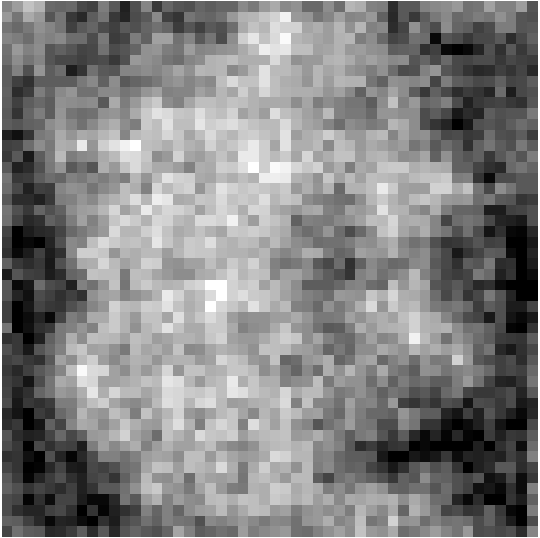
\includegraphics[scale=0.45]{reconstruction1_cropped}
		\caption{\small $P = 512$}
	\end{subfigure}%
	\begin{subfigure}[h]{0.45\textwidth}
		\centering
		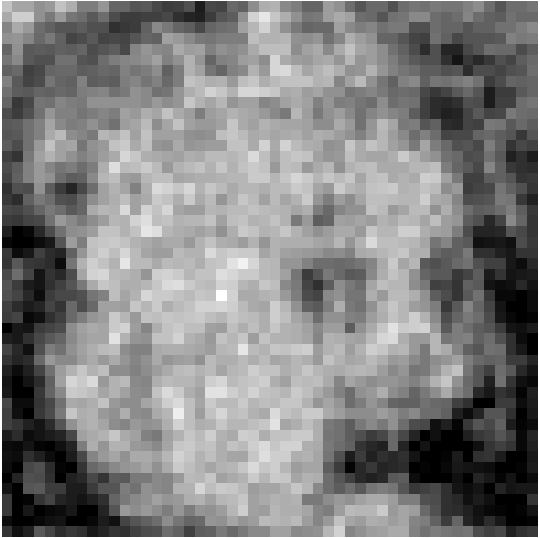
\includegraphics[scale=0.45]{reconstruction10_cropped}
		\caption{\small $P = 512\times 10$}
	\end{subfigure}%

		\begin{subfigure}[h]{0.45\textwidth}
		\centering
		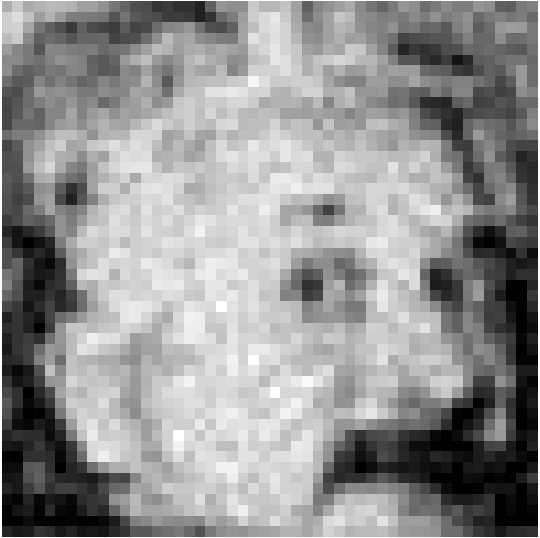
\includegraphics[scale=0.45]{reconstruction100_cropped}
		\caption{ \small $P = 512\times 10^2$ }
	\end{subfigure}%
	\begin{subfigure}[h]{0.45\textwidth}
		\centering
		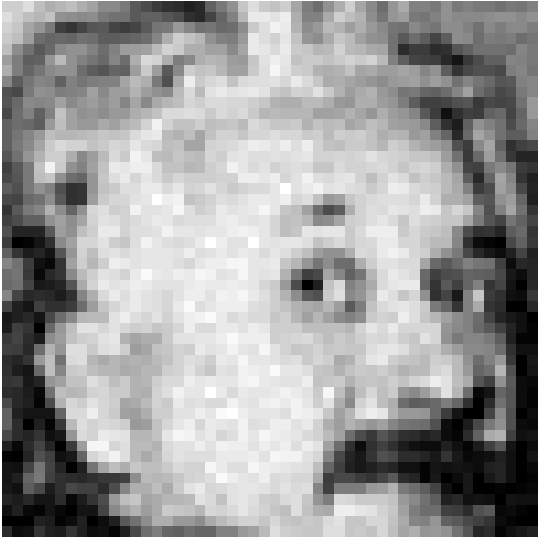
\includegraphics[scale=0.45]{reconstruction1000_cropped}
		\caption{\small $P = 512\times 10^3$}
	\end{subfigure}%

%	\begin{subfigure}[h]{0.33\textwidth}
%		\centering
%		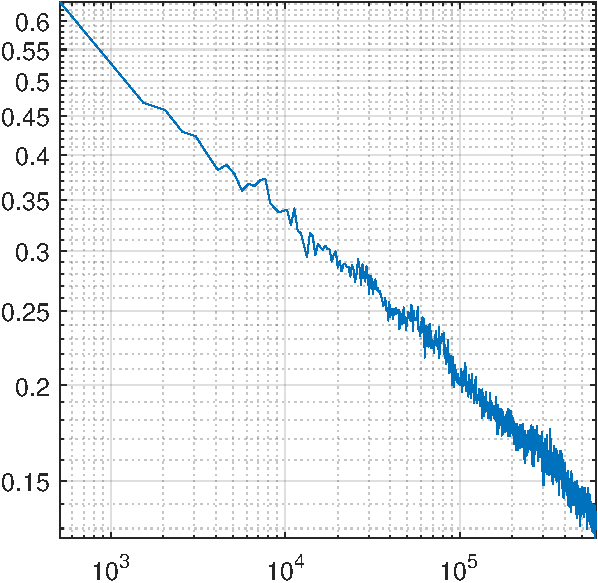
\includegraphics[scale=0.33]{Einstein_progress_cropped}
%		\caption{\label{fig:err_curve}\small Error curve}
%	\end{subfigure}%

%\begin{figure}[h!]
%	\centering
%	\begin{subfigure}[h]{0.25\textwidth}
%		\centering
%		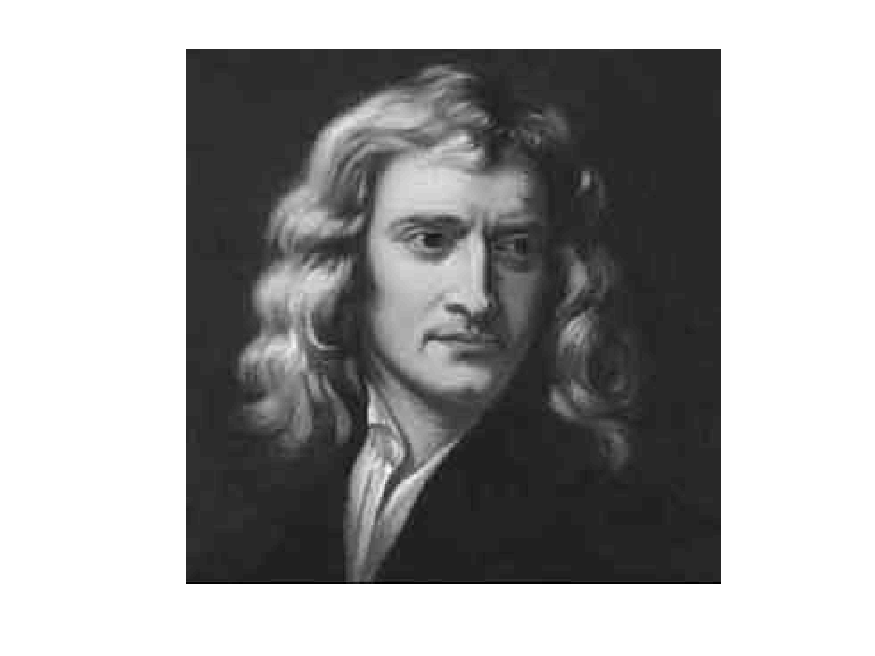
\includegraphics[scale=0.3]{Newton}
%		\caption{\label{fig:newton}Newton  (model)}
%	\end{subfigure}%
%	\begin{subfigure}[h]{0.25\textwidth}
%		\centering
%		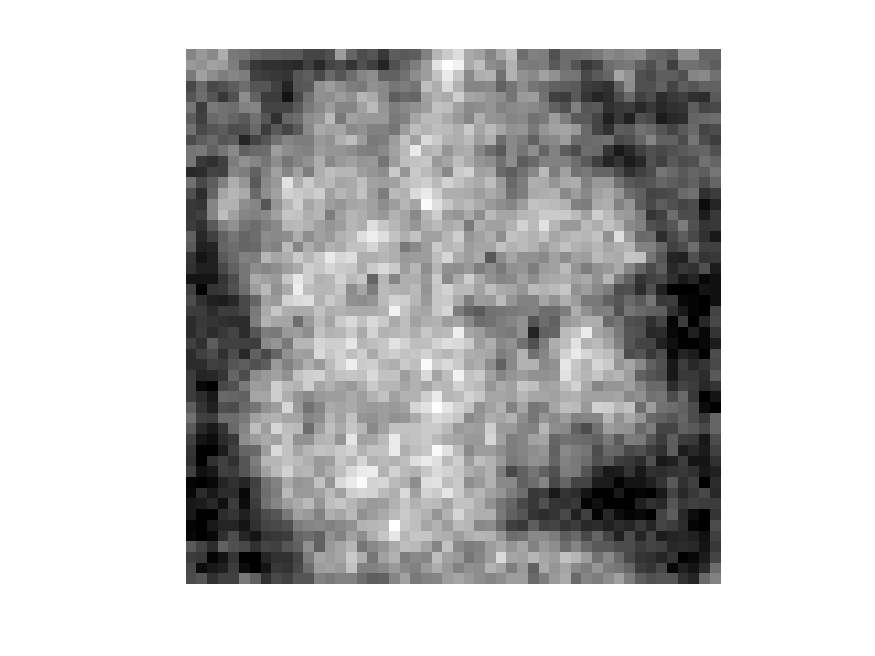
\includegraphics[scale=0.3]{reconstruction2}
%		\caption{\small $P =1024$}
%	\end{subfigure}%
%	\begin{subfigure}[h]{0.25\textwidth}
%		\centering
%		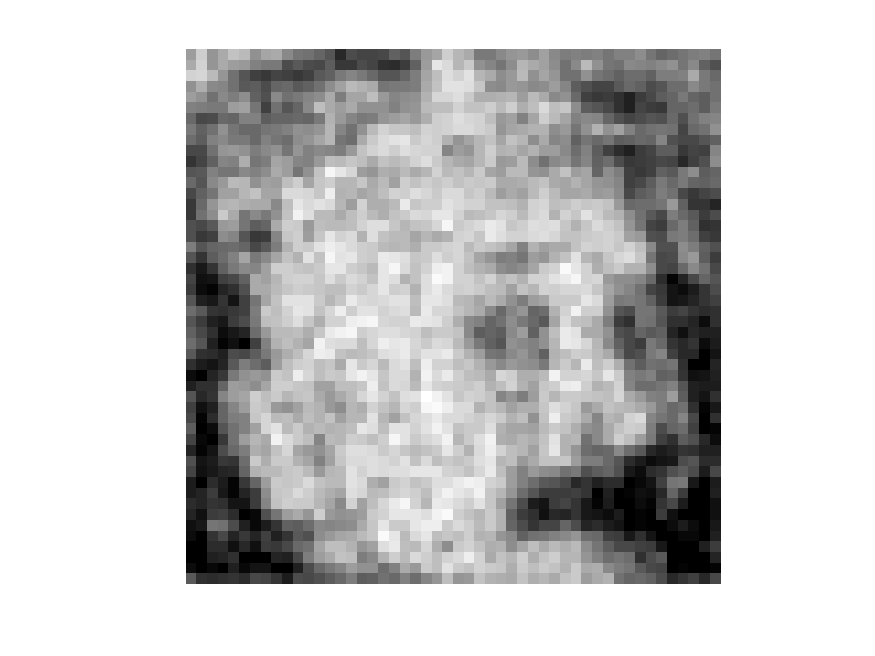
\includegraphics[scale=0.3]{reconstruction20}
%		\caption{$P = 1024\times 10$}
%	\end{subfigure}%
%	\begin{subfigure}[h]{0.25\textwidth}
%		\centering
%		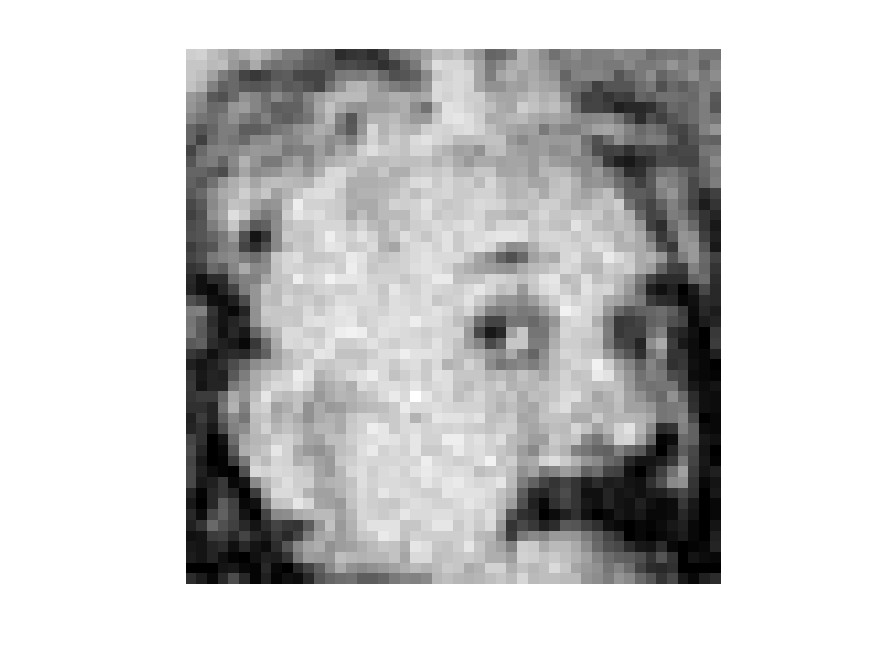
\includegraphics[scale=0.3]{reconstruction200}
%		\caption{$P = 1024\times 100$}
%	\end{subfigure}%
	\caption{\label{fig:Einst_example} Recovery of Einstein from micrographs at noise level $\sigma = 3$ (see Figure~\ref{fig:micro_example}(c)). Averaged autocorrelations of the micrographs allow to estimate the power spectrum of the target image. This does not require particle picking. A phase retrieval algorithm (RRR) produces the estimates here shown, initialized with an image of the physicist Isaac Newton. Estimates are obtained from $P$ micrographs (growing across panels), each containing $700$ image occurrences on average.---\TODO{Will add image with $P=512\times 10^4$ and image of Newton.}
		% At a noise level of $\sigma = 3$, this amounts to an $\SNR$ of $1/20$.
	}
\end{figure}



\begin{figure}[h]
\centering
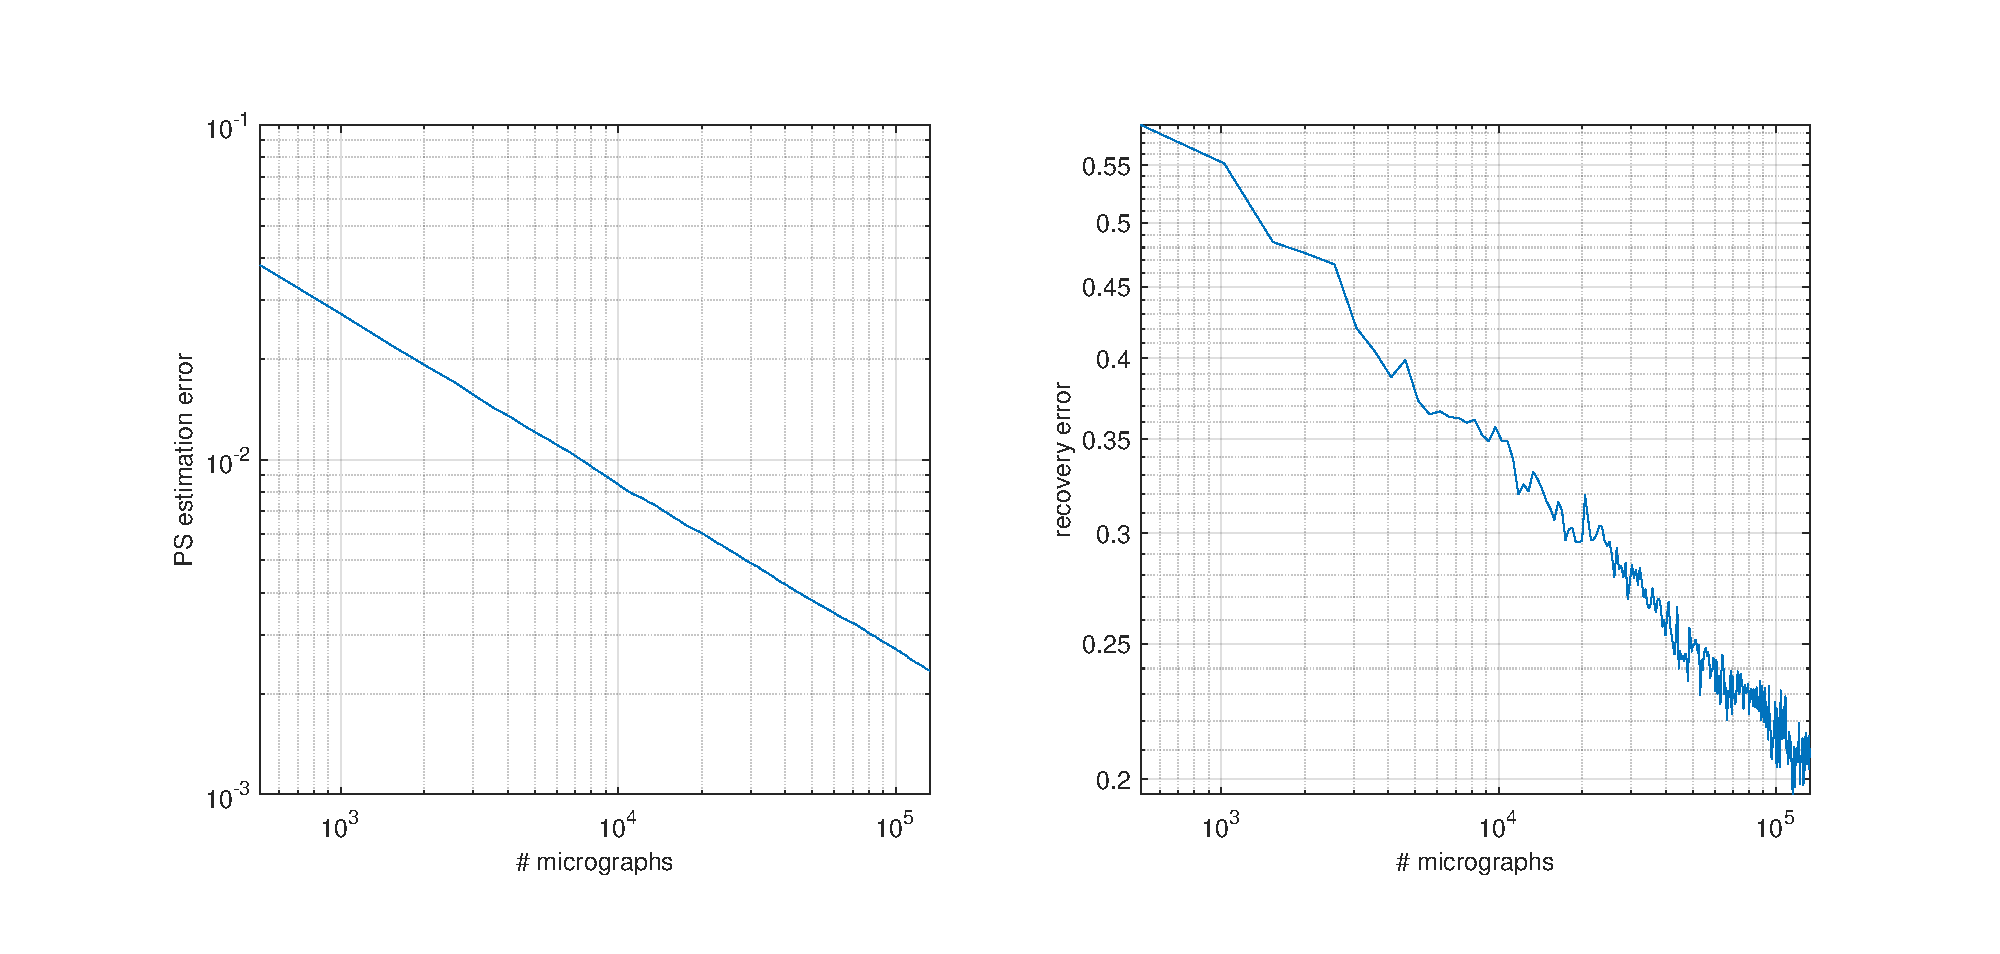
\includegraphics[scale=.7]{Einstein_progress}
\caption{\label{fig:error_per_micro} Relative root mean square error of the estimate of Einstein's image as a function of the number of observed micrographs (logarithmic scale along both axes.)}
\end{figure}



%
%Figure~\ref{fig:1Dheterosignals} demonstrates accurate estimation of three signals simultaneously with noise level $\sigma=3$. We define the ratio of the space occupied by the $i$th signal as 
%\begin{equation}
%\gamma_i = \frac{M_i L}{N},
%\end{equation}
%where $M_i$ is the signal's number of occurrences, $L$ is the length of the signal and $N$ is the micrograph length. In the experiment, we do not assume to know these ratios, neither the noise level $\sigma$. As can be seen, given enough signals occurrences, we can estimate accurately the signals. he estimation quality 
%is poorer than the other two signals, a phenomenon that can be explained using Proposition~\ref{prop:uniqueness}.


In the second experiment, three 1-D signals, each of length $L = 21$, appear at random locations in one long 1-D signal, which we call a micrograph by analogy. Any two occurrences are separated by at least 20 entries. The signals appear respectively about 30, 20 and 10 million times in a micrograph of length 12.3 billion. The micrograph is then contaminated with additive white Gaussian noise. This results in an $\SNR$ of about $1/9$, while about 10\% of the micrograph contains signal. Neither the number of occurrences nor the noise level $\sigma$ are known.

In the methods section, we detail how autocorrelations of the micrograph can be used to estimate weighted averages of the autocorrelations of the target signals. The individual signals and their relative densities are then estimated from autocorrelations up to order three by solving a nonlinear least-squares problem.

Figure~\ref{fig:1Dheterosignals} shows how the estimates improve as we see a larger and larger fraction of the micrograph (that is, as more and more data becomes available.) As is clear from the picture, despite the high noise level which would make it very challenging to locate the signal occurrences, the individual signals can be estimated accurately given enough data. Furthermore, the propensity of each signal can also be estimated.

%In order to estimate the signals, we computed the first three autocorrelation functions of the data and then estimated the signals and their corresponding $\gamma_i$ using a nonconvex least-squares. 
%As can be seen, given enough signal occurrences, we can estimate accurately the signals. 
%The estimation quality of the triangle signal is poorer than the other two signals, a phenomenon that is explained using Proposition~\ref{prop:uniqueness}.

%We do not assume the knowledge of the noise level. 
%Crucially, starting from the point of $n\approx10^8$, the RMSE of the signal estimation decreases linearly with slope $-1/2$---the expected estimation rate of the autocorrelation functions---implying the stability of the recovery algorithm. 
%
%\begin{figure}[t]
%	\centering
%	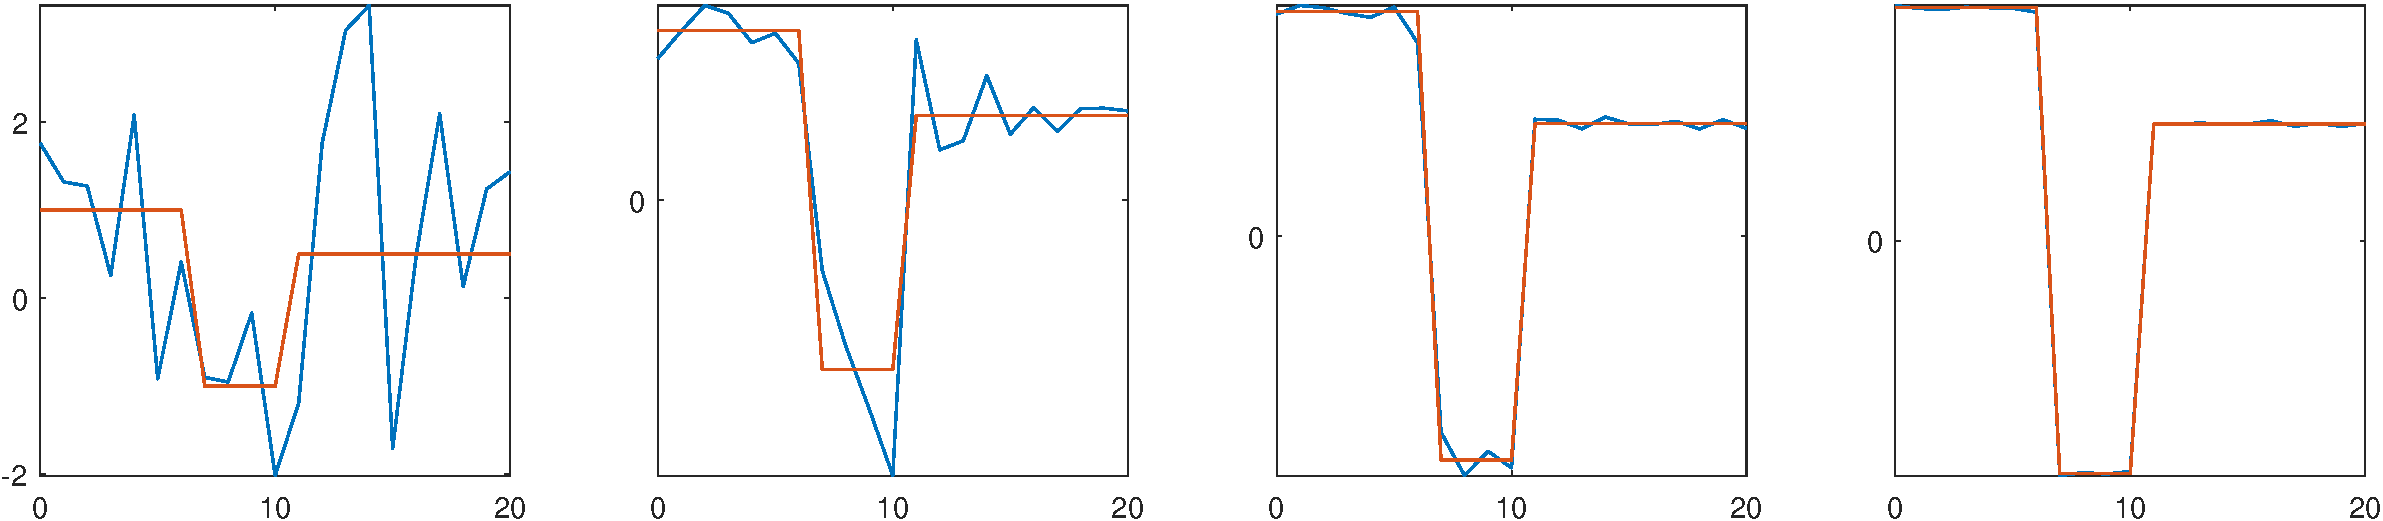
\includegraphics[scale=0.45]{progressive_n}
%	\caption{\TODO{...} \TODO{This figure is with new ROI method based on loss functions}}
%	\label{fig:1Dhomosignals}
%\end{figure}
%
%\begin{figure}[t]
%	\centering
%	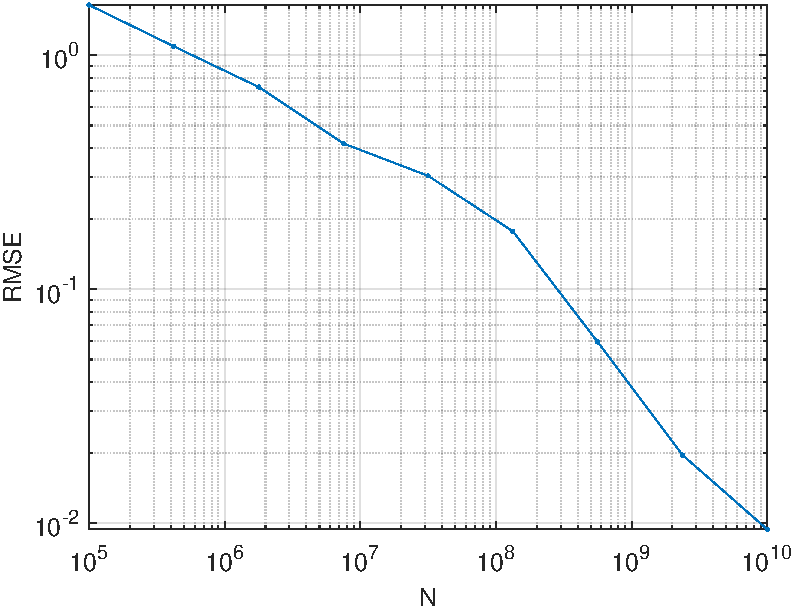
\includegraphics[width=0.5\linewidth]{XP_1D_homogeneous_new_ROI/progressive_RMSE_n}
%	\caption{\TODO{...} \TODO{This figure is with new ROI method based on loss functions}}
%	\label{fig:1DhomoRMSE}
%\end{figure}


\begin{figure}[t]
	\centering
	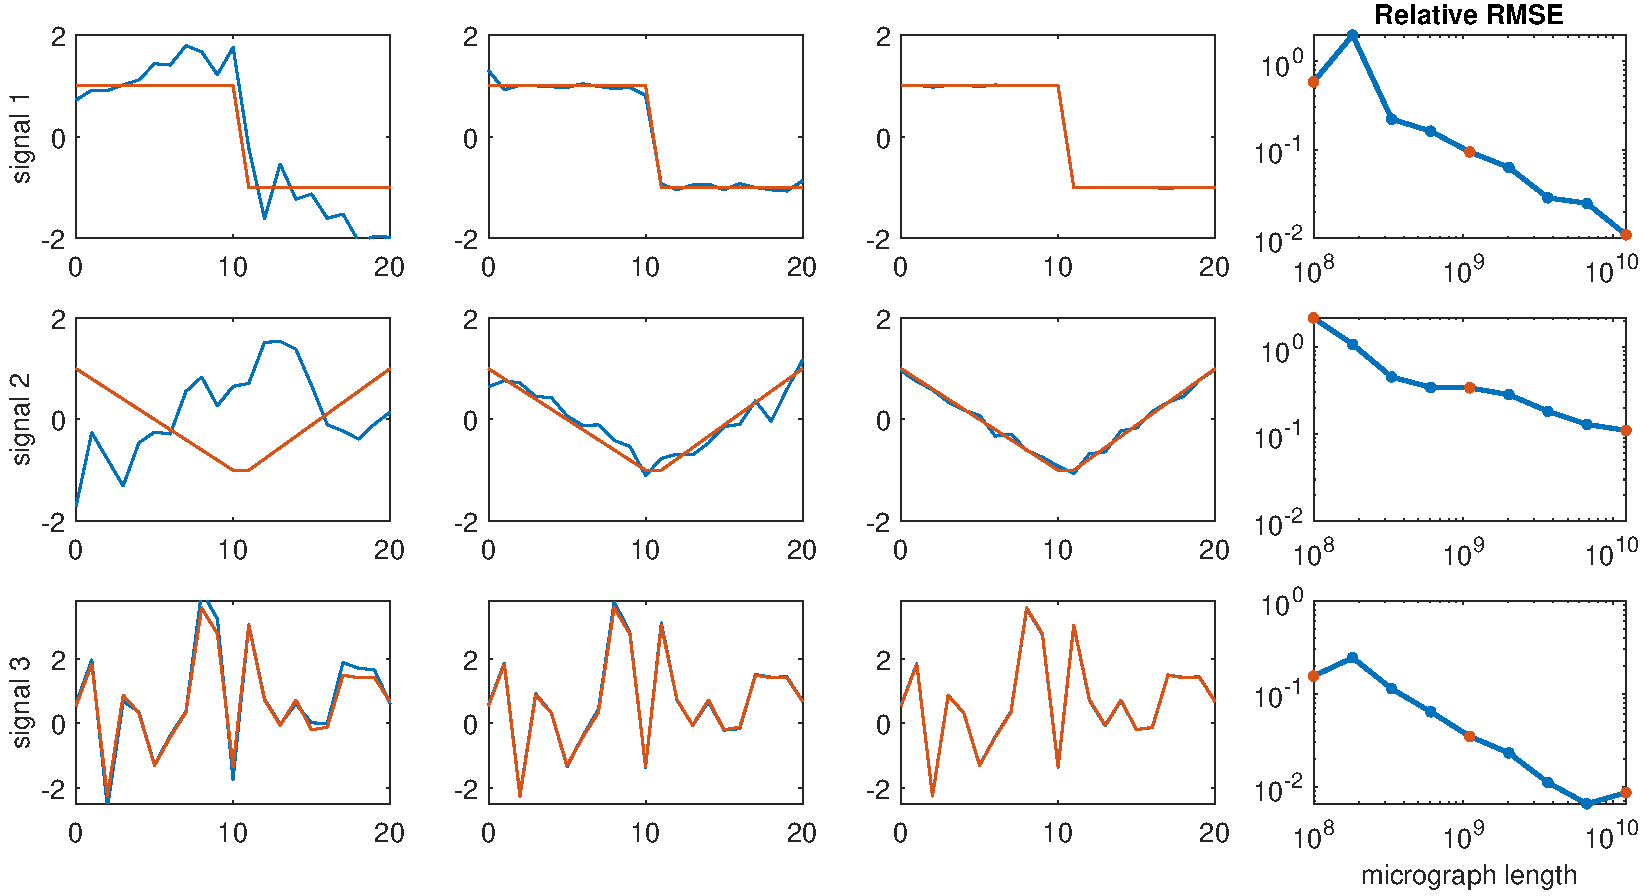
\includegraphics[width=\linewidth]{heterogeneous_progressive_n12300000000_466300}
	\caption{For the second experiment, each row shows, three times, one of the target signals (red), overlaid with an estimate (blue) obtained from a growing portion of the noisy micrograph (about $10^8$, $10^9$ and $10^{10}$ entries available to compute autocorrelations.) The last column depicts evolution of the relative root mean square error in estimating each individual target signal. Signals 1 to 3 appear respectively about 30.0, 20.0 and 10.0 million times. With the whole micrograph available, the algorithm estimated those to be 29.8, 21.9 and 10.0 million, respectively.
%		
%		An experiment for estimate three one-dimensional signals simultaneously with noise level $\sigma=3$. Red signals are the ground truth (targets) and the blue signals are our estimations. Individual RMSE of the estimates: $0.0239393 / 0.208925 / 0.0335956$. The estimated $\gamma$'s are $0.02574 / 0.01693 / 0.00818$ and the true ones $0.02561 / 0.01707 / 0.00853$. The $\SNR$ is $1/12$. \TODO{1. to replace with a ``progress'' plot 2. replace the triangle signal 3. add error progress figure}
	}
	\label{fig:1Dheterosignals}
\end{figure}



\clearpage
\section{Discussion}

%\TODO{Discussion: What might the answer imply and why does it matter? How does it fit in with what other researchers have found? What are the perspectives for future research?}

%All current algorithmic pipelines for SPR using cryo--EM start with a particle picking algorithm which is prone to model bias. 
%Bypassing the particle picking stage and constructing a 3-D model directly from the data---without assuming prior knowledge on the particle to be estimated---can be used to reconstruct ab initio models to initialize a refinement algorithm.  Alternatively, it can be applied to generate templates for a particle picker which does not suffer from model bias.


In the simplified model we examined, the aim is to estimate one, or possibly several, images from micrographs. Our strategy is to compute autocorrelation functions of the data and to relate these statistics to the unknown parameters. Recovering the parameters from the statistics reduces to solving a set of polynomial equations. Depending on the scenario, we did so using either a phase retrieval algorithm or a nonlinear least-squares algorithm.

The same general approach can, in principle, be applied directly to SPR from cryo-EM. Here, the micrographs contain numerous tomographic projections of molecules (possibly in different conformations) under unknown viewing directions. The aim is to estimate the 3-D volumes of the different conformations directly from micrographs. Each volume can be expanded linearly in a basis, so that the volume is characterized by its expansion coefficients. Since tomographic projection is a linear operation, autocorrelations of the micrographs (which can be estimated easily) are polynomial functions of the sought coefficients. Thus, autocorrelations of the micrographs provide a system of polynomial equations in the volume parameters, and the question becomes: are these equations sufficient to uniquely identify the volumes, and can we solve the system?

We show in Appendix~\ref{sec:cryoem} that the number of polynomial equations provided by the third-order autocorrelations is of the same order as the number of coefficients required to describe one volume at resolution comparable to that of the particle projections. This hints that it may be possible to reconstruct one or even several distinct volumes from these equations directly. Additional parameters in these equations could encode an unknown non-uniform viewing direction distribution and an unknown conformation distribution, which could then also be estimated. Crucially, the outlined approach involves no particle picking, hence a fortiori no viewing direction estimation or conformation clustering. As a result, it may not be limited to large molecules in the same way that particle picking approaches are. Concerns for model bias would also greatly be reduced.


%While the field is currently dominated by Bayesian methods such as EM, they are intractable for such problems. As an alternative, we propose to use autocorrelation analysis technique that shares some common lines (did you get the wordplay?)  with Kam's method for ab initio modeling~\cite{kam1980reconstruction,levin20173d,singer2018mathematics}. That being said, the SPR model is far more complicated than the model presented here. In a future research, we hope to bridge this gap.

Of course, we recognize that significant challenges lay ahead for the implementation of the proposed approach to 3-D reconstruction directly from the micrographs. We discuss a few now.

One possible concern is that the numerical experiments conducted here suggest a large amount of data may be necessary.\footnote{Whether or not this large amount of data would be necessary for any method to succeed given the unfavorable $\SNR$ is an interesting research question.} Recent trends in high-throughput cryo-EM technology \TODO{?} give hope that this may be a lesser concern in the long term. Still, large amounts of data also imply large amounts of computations. On this front, we note that computing autocorrelations of low orders can be done efficiently on CPUs and GPUs, and in parallel across micrographs. It can even be done in streaming mode, as only one look at each micrograph is necessary. The output of this data processing stage is a succinct summary in the form of autocorrelation estimates. Subsequent steps, which involve solving the system of polynomial equations, scale only in the size of that summary. Of course, an all important question then is whether the equations can be solved meaningfully in practice. The proof-of-concept experiments above suggest they might.

%Insofar as the computational challenges are concerned, we note that expectation-maximization algorithms (EM) have, over time, become the norm in the cryo-EM community, as exemplified by the popular RELION package. The idea of using EM for cryo-EM can be traced back at least to~\TODO{Sigworth}. At the time, such approaches also seemed challenging.


%\TODO{Do we want to say something about the number of images that we need? Specifically, do we want to address the fact that the numerical experiments suggest we may need a gigantic number of them for cryo, and mention trends in cryo technology that are encouraging in that regard? (Of course, we can't compare to RELION etc.\ in SNRs so low that one can't particle pick; that's not the point here.)}

Beyond data acquisition and computational challenges, there are modeling issues to consider.
As stated, our approach relies on two core assumptions that are not necessarily verified in SPR experiments.
First, we assume an additive white noise model, while in practice the noise may be structured or signal dependent. To address this point, it may be necessary to investigate better noise models and to extend the autocorrelation analysis accordingly.
Second, we assume that any two signal occurrences are sufficiently separated, and we use this assumption to derive algebraic relations between autocorrelations of the micrographs and autocorrelations of the target signals. 
Perhaps this separation could be induced by careful experimental design \TODO{?}.
Alternatively, if the signals are not well separated, one can introduce new parameters which encode the distribution of the spacing between occurrences. Here as well, relations between autocorrelation functions of the data and of the signals can be derived.
%Each variation leads to a different inverse problem. No sufficient conditions for them to be solvable are currently known.


\TODO{Do we want to note here that EM used to be perceived as computationally out of reach back when it was proposed [cite Fred], yet is now the de facto standard method as exemplified by RELION? Do we also want to stress that models have been refined over decades?}

\TODO{Should we discuss CTF? Where, and to what extent?}

\TODO{Where and how do we cite Kam? Fred?}

%The first entry $p[1]$ will represent the probability that two consecutive signals are separated by only one entry, $p[2]$ the probability for spacing of two entries and so on. Using this auxiliary variable $p$, one can write explicitly the relation between the autocorrelation functions of the data and those of the signal in a similar way to~\eqref{eq:data_ac}. 
%An interesting question is  under what conditions on $p$ and the signals, one can estimate the signals from the data.

\section{Methods} \label{sec:methods}


We derive algebraic relations between the autocorrelation functions of the micrographs and the autocorrelation functions of the target signals. For ease of exposition, we do so in the 1-D case. Extension to the 2-D case is straightforward. We also give additional technical details regarding the two experiments presented in Section~\ref{sec:results}.

Let $x_1,\ldots,x_K\in\RL$ be the sought signals and let $y\in\RN$ be the observed micrograph (notice that it is equivalent to think of the data as being one long micrograph or multiple shorter micrographs concatenated into one.)
The forward model (or ``image'' formation model) is as follows. For each target signal $x_k$, an unknown binary signal $s_k \in \{0, 1\}^{N-L+1}$ indicates (with 1's) the starting positions of all occurrences of $x_k$ in $y$, so that, with additive white Gaussian noise:
\begin{align}
	y & = \sum_{k=1}^K x_k \ast s_k + \varepsilon, & \varepsilon & \sim \mathcal{N}(0,\sigma^2 I_N),
	\label{eq:model}
\end{align}
where $\ast$ denotes (zero-padded) convolution. The binary signals obey the following property:
\begin{align}
	\textrm{If } s_k[i] = 1 \textrm{ and } s_{k'}[j] = 1 \textrm{ but } (k, i) \neq (k, j), \textrm{ then } |i - j| \geq 2L-1.
	\label{eq:spacing}
\end{align}
In words: the starting positions of any two occurrences (be it of the same signal or of two different signals) must be separated by at least $2L-1$ positions, so that their end points are necessarily separated by at least $L-1$ signal-free entries in the micrograph.

From $y$, we aim to recover $x_1, \ldots x_K$, and possibly also the number of occurrences of each. In contrast, particle picking is the task of estimating the binary signal $s = s_1 + \cdots + s_K$, while clustering is the task of separating $s$ into its components $s_1, \ldots, s_K$. Neither of the latter can be performed reliably if $\sigma$ is large (that is, at low $\SNR$.)

%We denote the set of these nonzero values by 
% $\mathcal{S}_i$ and its cardinality by $\vert \mathcal{S}_i\vert = M_i$. 
%By assuming that all $\mathcal{S}_i$'s are disjoint,  we let $s = \sum_{i=1}^Ks_i$, $\mathcal{S} = \bigcup_{i=1}^{K} \mathcal{S}_i$ and  $\vert \mathcal{S}\vert :=M =  \sum_{i=1}^{K}M_i$.  %Neither the $M_i$'s nor $M$ are assumed to be known.


Considering~\eqref{eq:model}, one can think of this inverse problem as a mixture of blind deconvolution problems between binary signals and the target signals. Related literature is briefly surveyed in Appendix~\ref{sec:related_literature}.

%In order to estimate the mixture of autocorrelations, we assume that the support of $s$ is not clustered. In particular, we assume that
%\begin{align}
%  \vert i-j \vert\geq 2L-1,   \quad \text{for all } i,j\in\mathcal{S} \text{ such that } i\neq j.
%  \label{eq:spacing}
%\end{align}
%The goal is to estimate $x_1,\ldots,x_K$ from $y$.


%
%\section{Autocorrelation analysis}   \label{sec:autocorrelation}
%
%Our method for estimating the signals is composed of two stages. 
%First, we use the autocorrelation functions of the data to estimate a mixture (i.e., linear combination) of the $K$ signal's autocorrelations. The mixed autocorrelation can be estimated to any accuracy, in any $\SNR$ level, if $M$ is large enough and the spacing condition~\eqref{eq:spacing} is met. Then, we  use a nonconvex LS  to estimate the signals from their mixed autocorrelations. 
%In this section, we elaborate on the autocorrelation functions and their estimations, while the precise recovery procedure, based on nonconvex optimization, will be discussed in detail in the next section.

\paragraph{Aperiodic autocorrelation functions}
%\subsection{Aperiodic autocorrelation functions} \label{sec:aperiodic_ac}

%\TODO{$L$ is a bad notation here since it could be L or n; and k is poor notation too because we use it to sum up to K.}

In general, for a signal $z$ of length $m$, the autocorrelation of order $q \geq 1$ is given for any integer shifts $\ell_1, \ldots, \ell_{q-1}$ by
\begin{align}
	a_z^q[\ell_1,\ldots,\ell_{k-1}]  & = \frac{1}{m} \sum_{i=-\infty}^{+\infty} z[i]z[i+\ell_1]\cdots z[i+\ell_{q-1}],
	\label{eq:ac_general}
\end{align}
where indexing of $z$ out of the range $0, \ldots, m-1$ is zero-padded.
For our purposes, this will be applied both to $x_k$'s (each of length $L$) and to $y$ (of length $N$).
Explicitly, the first-, second- and third-order autocorrelations are given by
\begin{align} 
	a_z^1 & = \frac{1}{m} \sum_{i=0}^{m-1} z[i], \nonumber\\
	a_z^2[\ell] & = \frac{1}{m} \sum_{i = \max\{0, -\ell\}}^{m-1 + \min\{0, -\ell\}} z[i]z[i+\ell], \nonumber\\
	a_z^3[\ell_1,\ell_2] & = \frac{1}{m} \sum_{i = \max\{0, -\ell_1, -\ell_2\}}^{m-1 + \min\{0, -\ell_1, -\ell_2\}} z[i]z[i+\ell_1]z[i+\ell_2]. \label{eq:ac_special}
\end{align}
The autocorrelation functions have symmetries. Specifically, $a_z^2[\ell] = a_z^2[-\ell]$, and
\begin{align*}
	a_z^3[\ell_1,\ell_2] = a_z^3[\ell_2,\ell_1]=a_z^3[-\ell_1,\ell_2-\ell_1].
\end{align*}
%Additionally, if the moments of the signal depend only on the difference between the indices (Toeplitz structure), then they are equivalent to the autocorrelation functions.
Taking these symmetries into consideration, one can show that $a_z^1, a_z^2$ and $a_z^3$ contain \TODO{TKTK} (respectively) non-trivial distinct real numbers, generically.

\paragraph{Estimating the autocorrelation function of a single signal.}

For the special case $K = 1$ where a single signal $x = x_1$ must be recovered, the relation between autocorrelations of the micrograph and those of $x$ is particularly simple, so that we treat it first. It is useful to introduce some notation: let $M$ denote the number of occurrences of $x$ in $y$, and let
\begin{align}
	\gamma & = \frac{M L}{N}
\end{align}
denote the density of $x$ in $y$ (that is, the fraction of entries of $y$ occupied by occurrences of $x$.) The spacing constraint~\eqref{eq:spacing} imposes $\gamma\leq\frac{L}{2L-1}\approx 1/2$.

One simple observation is that the first-order autocorrelation of $y$ (its mean) is independent of the locations of $x$. Since the noise is independent of the signal, the mathematical expectation of $a_y^1$ is easily seen to be:\footnote{We did not fully specify a random generating model for the location vector $s$. The expectation is still well defined specifically because the quantity under consideration is independent of $s$ under the assumptions.}
\begin{align*}
	\E\{ a_y^1 \} & = \gamma a_x^1.
\end{align*}
We consider the asymptotic regime where $M, N\to\infty$, while $\gamma$ remains constant (we see an increasingly large micrograph, containing increasingly many signal occurrences, with constant signal density.) In that regime, the law of large numbers gives meaning to the following statement:
\begin{align*}
	\lim_{N\to\infty} a_y^1 & = \gamma a_{x}^1.
\end{align*}
Thus, given enough data, if $\gamma$ is known, we can estimate $a_x^1$ from $y$. (We show later how to estimate $\gamma$ as well.)

The spacing constraint~\eqref{eq:spacing} gives rise to more powerful observations. Consider the second-order autocorrelation in particular: $a_y^2[\ell]$ computes the correlation between $y$ and a copy of $y$ shifted by $\ell$ entries. Considering $\ell$ only in the range $0, \ldots, L-1$, one can see that any given occurrence of $x$ in $y$ is only ever correlated with itself (with the same shift $\ell$), and never with another occurrence. As a result,
\begin{align*}
	\lim_{N\to\infty} a_y^2[\ell] & = \gamma a_{x}^2[\ell] + \sigma^2\delta[\ell]
\end{align*}
for $\ell = 0, \ldots, L-1$, where $\delta$ denotes the Kronecker delta function. The last part captures the autocorrelation of the noise. Notice that, even if $\sigma$ is unknown, entries $\ell = 1, \ldots, L-1$ still provide useful information about $a_x^2$.
Along the same lines, one can establish a relation for third-order autocorrelations:
\begin{align}
	\lim_{N\to\infty} a_y^3[\ell_1,\ell_2] & = \gamma a_{x}^3[\ell_1,\ell_2] + \sigma^2\gamma a_{x}^1 \cdot \big(\delta[\ell_1,0]+\delta[0,\ell_2]+\delta[\ell_1,\ell_2]\big),
	\label{eq:data_ac_k1}
\end{align}
for $\ell_1,\ell_2 = 0, \ldots, L-1$. Here too, few entries are affected by $\sigma$ in the limit.
Detailed derivations for identities in this and the next part are given in Appendix~\ref{sec:autocorrelation_computation}.

\paragraph{Estimating the autocorrelation function of multiple signals.}

Returning to the general case $K \geq 1$, let $M_1, \ldots, M_K$ denote the number of occurrences of signals $x_1, \ldots, x_K$ respectively, and define
\begin{align}
	\gamma_k & = \frac{M_k L}{N}, & \gamma & = \sum_{k=1}^K\gamma_k.
\end{align}
As above, we consider the asymptotic regime where $M_1,\ldots,M_K,N\to\infty$ while preserving the ratios $\gamma_k$ constant.
% 
Still under the spacing constraint~\eqref{eq:spacing}, similarly to the developments above, one can estimate a mixture of the autocorrelations of the $K$ target signals from the autocorrelations of the micrograph:
\begin{align}
\lim_{N\to\infty} a_y^1 & = \sum_{k=1}^K\gamma_k a_{x_k}^1, \nonumber\\
\lim_{N\to\infty} a_y^2[\ell] & = \sum_{k=1}^K\gamma_k a_{x_k}^2[\ell] +\sigma^2\delta[\ell],  \label{eq:data_ac}\\
\lim_{N\to\infty} a_y^3[\ell_1,\ell_2] & = \sum_{k=1}^K\gamma_k a_{x_k}^3[\ell_1,\ell_2] + \sigma^2\left(\sum_{k=1}^K\gamma_k a_{x_k}^1\right)(\delta[\ell_1,0]+\delta[0,\ell_2]+\delta[\ell_1,\ell_2]), \nonumber
\end{align}
where $\ell, \ell_1, \ell_2 = 0, \ldots, L-1$. The left hand side is straightforward to estimate from data: it provides a succinct summary of it. The right hand side involves polynomial functions of unknowns $\gamma_1, \ldots, \gamma_K, x_1, \ldots, x_K$. The task is to solve these polynomial equations in a robust way.

\paragraph{First numerical experiment.}
For the 2-D experiment shown in Figures~\ref{fig:Einst_example} and~\ref{fig:error_per_micro}, we generated $P$ micrographs of size $4096\times 4096$ pixels. 
In each micrograph, we placed Einstein's image of size $50\times 50$  in random locations, while keeping the separation condition~\eqref{eq:spacing}.  
This is done by randomly selecting $4000$ placements in the micrograph, one at a time with
an accept/reject rule based on the separation constraint and locations picked so far. On average, $700$ images were placed in each micrograph.   
Then, an i.i.d.\ Gaussian noise with standard deviation $\sigma=3$ was added inducing $\SNR$ of approximately $1/20$. An example of a micrograph's excerpt is presented in the right panel of Figure~\ref{fig:micro_example}.
%Different micrographs are handled sequentially on a GPU, as GPUs are particularly well suited to execute simple instructions across large vectors of data. If multiple GPUs are available, segments can of course be handled in parallel.


In this experiment, we assume to know the number of Einstein's occurrences and the noise level. 
In this situation, the second-order autocorrelation (or, equivalently, the Fourier magnitudes of the signal) determines  almost all images  uniquely up to reflection through the origin~\cite{hayes1982reconstruction,bendory2017fourier}. 
Therefore, we estimate the signal's Fourier magnitude from the Fourier magnitude of the micrographs, in the cost of one  FFT per micrograph.
To estimate the signal, we use a phase retrieval algorithm called relaxed-reflect-reflect (RRR) that iterates by
\begin{equation}
z \rightarrow z + \beta (P_2(2P_1(z) - z) - P_1(z)),
\end{equation}
where we set $\beta=1$.
RRR estimates a $2L\times 2L$ image. Exact solution contains Einstein's image in the upper-left corner and zero else where. The operator $P_2(z)$ combines the Fourier phases of  the current estimation $z$ with the Fourier magnitudes of the signal  (estimated from the data). The operator $P_1(z)$ zeros out all entries of $z$ outside the $L\times L$ upper-left corner. 
In order to compare the performance in multiple cases and different noise levels, the algorithm stopped after a fixed number of 1000 iterations and the iteration with the smallest error compared to the ground truth (also taking into account the reflection ambiguity) was chosen as the solution. While this cannot be done in practice since we do not have access to the ground truth, this procedure enables us to compare a large number of instances in different noisy environments \TODO{Note the last two sentences!}.

\paragraph{Second numerical experiment.}
For the 1-D experiment, we worked with three signals of length $L = 21$ and generated the data in the same way as in the 2-D example.
The only difference is that here, for each
placement, one of the three signals is picked at random proportionally to the desired number
of occurrences of each.
In this experiment, we computed the first three autocorrelation functions. 
We do not assume to know the number of occurrences of each signal $\gamma_i$ ahead and we removed the biased terms (see~\eqref{eq:data_ac_k1}) so we do not need to know $\sigma$ either. 
\TODO{In Appendix~\ref{sec:theory} we provide an argument on the number of equations we get from the first three autocorrelation functions. -- Was this removed? I can't find it.}

To estimate the signal, we use an optimization algorithm on the following nonlinear least-squares problem that estimates the signals and their density of occurrences simultaneously:
\begin{multline}
\min_{\substack{\hat x_1, \ldots, \hat x_K \in \reals^{W} \\ \hat \gamma_1, \ldots, \hat \gamma_K > 0}} w_1 \left( a_y^1 - \sum_{k=1}^K \hat \gamma_k a_{\hat x_k}^1 \right)^2 + w_2 \sum_{\ell = 1}^{L-1} \left( a_y^2[\ell] - \sum_{k=1}^K \hat \gamma_k a_{\hat x_k}^2[\ell] \right)^2 + \\ w_3 \sum_{\substack{2\leq\ell_1\leq L-1 \\ 1 \leq \ell_2 \leq \ell_1-1}} \left( a_y^3[\ell_1, \ell_2] - \sum_{k=1}^K \hat \gamma_k a_{\hat x_k}^3[\ell_1,\ell_2] \right)^2.
\label{eq:optim1D}
\end{multline}
where $W \geq L$ is the length of the sought signals and $w_1 = \frac{1}{2}, w_2 =\frac{1}{2}(L-1), w_3 = \frac{1}{(L-1)(L-2)}$; see~\cite{boumal2017heterogeneous} see for discussion on how to choose the weights properly.


 Setting $W = L$ (as is a priori desired) is problematic because the above optimization problems appears to have numerous poor local optimizers.
%Since we can only initialize randomly at first, this approach would often fail in practice. Alternatively,
Thus, we first run the optimization with $W = 2L-1$. This problem appears to have fewer poor local optima, perhaps because the additional degrees of freedom allow for more escape directions. Since we hope the signals estimated this way correspond to the true signals zero-padded to length $W$, we extract from each one a subsignal of length $L$ whose autocorrelation functions are closest to the measured ones in the sense of~\eqref{eq:optim1D}. 
This estimator is then used as initial iterate for~\eqref{eq:optim1D}, this time with $W = L$. We find that this procedure is reliable for a wide range of experimental parameters. To solve~\eqref{eq:optim1D}, we run the trust-region method implemented in Manopt~\cite{manopt}, which allows to treat the positivity constraints \TODO{reference} on coefficients $\hat \gamma_k$. Notice that the cost function is a polynomial in the variables, so that it is straightforward to compute it and its derivatives.



%For the 1-D experiment, we fix $K = 3$ signals of length $L = 21$, as depicted in Figure~\TODO{ref}. Following the data model described in Section~\TODO{ref}, we generate an observation $y$ of length $24.6 \cdot 10^9$. Each of the three signals appears, respectively (and approximately) $300 \cdot 10^6$, $200 \cdot 10^6$ and $100 \cdot 10^6$ times in $y$, such that at least $L-1$ zeros separate two occurrences of any signals. 
%This is done by randomly selecting $600 \cdot 10^6$ placements in $y$, one at a time with an accept/reject rule based on the separation constraint and locations picked so far. For each placement, one of the three signals is picked at random proportionally to the desired number of occurrences of each. Then, i.i.d.\ Gaussian noise with mean zero and standard deviation $\sigma = 3$ is added, to form the observed $y$. The SNR of $y$
% sqrt((m_want*sum(X.^2)')/(sigma^2*n))
%is about 1/12.


%This is enough noise to make cross-correlations of $y$ even with the true signals display peaks at random locations, uninformative of the actual locations of the signal occurrences. Thus, we contend that it would be difficult for any algorithm to locate the signal occurrences, let alone to classify them according to which signal appears where.

%\TODO{TB: I would place the equation counting argument in the theory section in the paragraph of open questions (I marked th place)}
%
%Given the observation $y$, we proceed to compute the moments. The first-order moment is straightforward. For second-order moments, notice from equation~\eqref{eq:data_ac} that $a_y^2[\ell]$ suffers no bias for $\ell$ in $1$ to $L-1$. Thus, we omit $\ell = 0$, which has the practical effect that we need not know $\sigma$ to estimate the moments. Likewise, for third-order moments, $a_y^3[\ell_1, \ell_2]$ for $0 \leq \ell_1, \ell_2 \leq L-1$ such that $\ell_2 \leq \ell_1$ includes all relevant moments for our purpose \TODO{Do we want to include a figure to explain why that is?}, and we further exclude any such that $\ell_1, \ell_2$ or $\ell_1 - \ell_2$ are zero to avoid biased elements---there are $\frac{(L-1)(L-2)}{2}$ remaining moments. As a result, it is unnecessary to estimate $\sigma$. We have \TODO{TB: We may want to put this calculation is the last paragraph of Section 3.1 }
%\begin{align*}
%1 + (L-1) + \frac{(L-1)(L-2)}{2} = \frac{1}{2} L (L-1) + 1
%\end{align*}
%moments in total. In practice, these are computed on disjoint segments of $y$ of length $100\cdot10^6$ and added up, without correction for the junction points. Segments are handled sequentially on a GPU, as GPUs are particularly well suited to execute simple instructions across large vectors of data. If multiple GPUs are available, segments can of course be handled in parallel.
%
%Having computed the moments of interest, we now estimate signals $x_1, \ldots, x_K$ and coefficients $\gamma_1, \ldots, \gamma_K$ which agree with the data. We choose to do so by running an optimization algorithm on the following nonlinear least-squares problem:
%\begin{multline}
%\min_{\substack{\hat x_1, \ldots, \hat x_K \in \reals^{W} \\ \hat \gamma_1, \ldots, \hat \gamma_K > 0}} w_1 \left( a_y^1 - \sum_{k=1}^K \hat \gamma_k a_{\hat x_k}^1 \right)^2 + w_2 \sum_{\ell = 1}^{L-1} \left( a_y^2[\ell] - \sum_{k=1}^K \hat \gamma_k a_{\hat x_k}^2[\ell] \right)^2 + \\ w_3 \sum_{\substack{2\leq\ell_1\leq L-1 \\ 1 \leq \ell_2 \leq \ell_1-1}} \left( a_y^3[\ell_1, \ell_2] - \sum_{k=1}^K \hat \gamma_k a_{\hat x_k}^3[\ell_1,\ell_2] \right)^2.
%\label{eq:optim1D}
%\end{multline}
%where $W \geq L$ is the length of the sought signals and \TODO{explain $w_i$'s: currently they are $w_1 = 1/2, w_2 = 1/2n_2, w_3 = 1/2n_3$, where $n_2, n_3$ are the number of moments used: $n_2 = L-1$, $n_3 = \frac{(L-1)(L-2)}{2}$. Issue is: this is not very smart..}. Setting $W = L$ (as is a priori desired) is problematic because the above optimization problems appears to have numerous poor local optimizers.
%%Since we can only initialize randomly at first, this approach would often fail in practice. Alternatively,
%Thus, we first run the optimization with $W = 2L-1$. This problem appears to have fewer poor local optima, perhaps because the additional degrees of freedom allow for more escape directions. Since we hope the signals estimated this way correspond to the true signals zero-padded to length $W$, we extract from each one a subsignal of length $L$ (with cyclic indexing \TODO{we should understand / explain this}) that has largest $\ell_2$-norm. This estimator is then used as initial iterate for~\eqref{eq:optim1D}, this time with $W = L$. We find that this procedure is reliable for a wide range of experimental parameters. To solve~\eqref{eq:optim1D}, we run the trust-region method implemented in Manopt~\cite{manopt}, which allows to treat the positivity constraints \TODO{I might need a reference for this} on coefficients $\hat \gamma_k$. Notice that the cost function is a polynomial in the variables, so that it is straightforward to compute it and its derivatives.
%\TODO{Should we do variable projection for the gammas, that is, exploit the fact the problem is a regular least squares in the gammas (up to the positivity constraints) to substitute the explicit optimum for them? Not sure it's worth the effort. -- Ok, it's probably not a good idea, because even with fixed gammas to the correct value, optimization takes a while.}
%\TODO{Do we still need to stress at this point that the optimization part has complexity independent of length of observation? Should be pretty clear at this point already.}
%
%



\bibliographystyle{plain}
\bibliography{ref}



\appendix

\section{Proof of \eqref{eq:data_ac}} \label{sec:autocorrelation_computation}

Throughout the proof, we consider the case of one signal $K=1$. The extension to $K>1$ is straightforward by averaging the contributions of all signal with  appropriate weights; see~\cite{boumal2017heterogeneous}. 

We will let the number of instances of the signal $M$ grow with $N$, and write $M=M_N$ to emphasize this. We assume $M_N$ grows proportionally with $N$, and define:
%
\begin{equation}
\gamma = \lim_{N\to\infty} \frac{M_NL}{N}<1.
\end{equation}
%
We will assume that $M_N=\Omega(N)$, so that $\gamma>0$. In the sequel, we will suppress the explicit dependence of $M$ on $N$ for notational convenience.

We start by considering the mean of the data:
%
\begin{equation}
a_y^1 = \frac{1}{N}\sum_{i=0}^{N-1} y[i] =
\frac{1}{N/L}\sum_{j=0}^{M-1}\frac{1}{L}\sum_{i=0}^{L-1}x[i] +    
\underbrace{\frac{1}{N}\sum_{i=0}^{N-1}\varepsilon[i]}_{\text{noise term}}
\xrightarrow{a.s.}\gamma a_x^1,
\end{equation}
%
where the noise term converges to zero almost surely (a.s.) by the strong law of large numbers.

We proceed with the (second-order) autocorrelation for fixed $\ell\in[0,\ldots,L-1]$. We can compute:
%

\begin{align}
%
a_y^2[\ell] & = \frac{1}{N}\sum_{i=0}^{N-1-\ell}y[i]y[i+\ell]
\nonumber \\
& = \underbrace{\frac{1}{N}\sum_{j=1}^{M}\sum_{i=0}^{L-\ell-1}x[i]x[i+\ell]}_{\text{signal term}} + \underbrace{\frac{1}{N}\sum_{i=0}^{N-1-\ell}\varepsilon[i]\varepsilon[i+\ell]}_{\text{noise term}}
+ \underbrace{\frac{1}{N} \sum_{j=1}^{M} \sum_{i=0}^{L-1} x[i] \varepsilon[s_j + i + \ell]}_{\text{cross-term}}.
%
\end{align}

The cross-terms are linear in the noise, and are easily shown to vanish almost surely in the limit $N\to\infty$, by the strong law of large numbers. As for the signal term, we break it into $M$ different sums, each containing one copy of the signal. This gives:
%
\begin{equation} \label{eq:2nd_moment_signal_term}
%
\frac{1}{N}\sum_{j=1}^{M}\sum_{i=0}^{L-\ell-1}x[i]x[i+\ell] = \frac{ML}{N}\frac{1}{L}\sum_{i=0}^{L-\ell-1}x[i]x[i+\ell]\xrightarrow{N\to\infty}\gamma a_x^2[\ell].
%
\end{equation}
%

We next analyze the pure noise term. When $\ell\neq 0$, we can break the noise term into a sum of independent terms:
%
\begin{equation}
%
\frac{1}{N}\sum_{i=0}^{N-1-\ell} \varepsilon[i]\varepsilon[i+\ell] = \frac{1}{\ell}\sum_{i=0}^{\ell-1}\frac{1}{N/\ell}\sum_{j=0}^{N/\ell -1} \varepsilon[j\ell + i] \varepsilon[(j+1)\ell + i].
%
\end{equation}
%
Each sum $\frac{1}{N/\ell}\sum_{j=0}^{N/\ell -1} \varepsilon[j\ell + i] \varepsilon[(j+1)\ell + i]$ is an average of $N/\ell$ independent terms with expectation zero, and thus converges to zero almost surely as $N\to\infty$. If $\ell=0$, then we have:
%
\begin{equation}
%
\frac{1}{N}\sum_{i=0}^{N-1} \varepsilon^2[i] \xrightarrow{a.s.} \sigma^2.
%
\end{equation}

We now analyze the third-order autocorrelation. Let us fix $\ell_1\geq\ell_2\ge0$. We have:
%
\begin{align}
%
&a_y^3[\ell_1,\ell_2] 
= \frac{1}{N}\sum_{i=0}^{N-1-\ell_1} y[i]y[i+\ell_1]y[i+\ell_2]
\nonumber \\
%
=& \underbrace{ \frac{ML}{N}\frac{1}{M}\sum_{j=1}^M 
	\frac{1}{L}\sum_{i=0}^{L-1-\ell_1}x[i]x[i+\ell_1]x[i+\ell_2]   }_{(1)}
+ \underbrace{\frac{1}{N}\sum_{i=0}^{N-1-\ell_1} \ep[i]\ep[i+\ell_1]\ep[i+\ell_2]}_{(2)}
\nonumber \\
&+ \underbrace{\frac{1}{N}\sum_{j=1}^{M} 
	\sum_{i=0}^{L-1} x[i]\ep[s_j + i+\ell_1]\ep[s_j+ i+\ell_2]}_{(3)}
+ \underbrace{\frac{1}{N}\sum_{j=1}^{M} 
	\sum_{i=0}^{L-1} \ep[s_j+i-\ell_1]x[i]\ep[s_j+ i+\ell_2-\ell_1]}_{(4)}
\nonumber \\
&+ \underbrace{\frac{1}{N}\sum_{j=1}^{M} 
	\sum_{i=0}^{L-1} \ep[s_j+i-\ell_2]\ep[s_j+i+\ell_1-\ell_2]x[i]}_{(5)}
+ \underbrace{\frac{1}{N}\sum_{j=1}^{M} 
	\sum_{i=0}^{L-\ell_1+\ell_2-1} \ep[s_j+i]x[i+\ell_1-\ell_2]x[i]}_{(6)}
\nonumber \\
&+ \underbrace{\frac{1}{N}\sum_{j=1}^{M} 
	\sum_{i=0}^{L-\ell_2-1} x[i]\ep[s_j + i+\ell_1]x[s_j+ i+\ell_2]}_{(7)}
+ \underbrace{\frac{1}{N}\sum_{j=1}^{M} 
	\sum_{i=0}^{L-\ell_1-1} x[i]x[i+\ell_1]\ep[s_j+ i+\ell_2]}_{(8)}.
%
\end{align}
%
Terms (6), (7) and (8) are linear in $\ep$, and can easily be shown to converge to 0 almost surely by the law of large numbers, by similar arguments as used previously. Term (1) converges to $\gamma a_x^3[\ell_1,\ell_2]$ almost surely, for the same reasons as~\eqref{eq:2nd_moment_signal_term}. To deal with terms (2)--(5), we must distinguish between different values of $\ell_1$ and $\ell_1$.

{\bf Case 1:} $0 < \ell_2 < \ell_1$. Here, all summands with elements of $\ep$ involve products of distinct entries, which have expected value 0. Consequently, the usual argument shows that terms (2)--(5) all converge to 0 almost surely as $N \to \infty$.

{\bf Case 2:} $0=\ell_2 < \ell_1$. Term (2) is an average of products of the form $\ep[i]^2\ep[i+\ell_1]$, which have mean zero; consequently, term (2) converges to 0 almost surely. The same argument as for Case 1 shows that (3) and (5) also converge to 0. For term (4), we write:
%
\begin{align}
%
&\frac{1}{N}\sum_{j=1}^{M} 
\sum_{i=0}^{L-1} \ep[s_j+i-\ell_1]x[i]\ep[s_j+ i+\ell_2-\ell_1]
\nonumber \\
&= \frac{ML}{N}\frac{1}{L}\sum_{i=0}^{L-1}x[i] \frac{1}{M}\sum_{j=1}^{M} \ep[s_j+i-\ell_1]^2
\xrightarrow{N\to\infty} \gamma \frac{1}{L} \sum_{i=0}^{L-1}x[i] \sigma^2 = \gamma a_x^1 \sigma^2.
%
\end{align}

{\bf Case 3:} $0<\ell_2 = \ell_1$. An argument nearly identical to that for Case 2 shows that terms (2), (4) and (5) converge to 0, while term (3) converges to $\gamma a_x^1 \sigma^2$.

{\bf Case 4:} $0=\ell_2 = \ell_1$. The same argument as for term (4) in Case 2 shows that terms (3), (4) and (5) all converge to $\gamma a_x^1 \sigma^2$. Term (2) is an average of $\ep[i]^3$, which is mean zero; consequently, it converges to 0.


This completes the proof of \eqref{eq:data_ac}.






\begin{comment}
Writing explicitly in terms of signal and noise, the sum can be broken into eight terms. The first contains only signal terms (does not see noise) and converges to $\gamma a_x^3$ from the same reasons as~\eqref{eq:2nd_moment_signal_term}. Three other terms contain the product of two signal entries and one noise term. Since the noise is independent of the signal and has zero mean, these terms go to zero almost surely.

We next analyze the contribution of the term composed of triple products of noise terms. For $\ell_1\neq 0$, this sum can be formulate as follows:
\begin{equation*}
\sum_{i=0}^{N-1-\ell_1} \varepsilon[i]\varepsilon[i+\ell_1]\varepsilon[i+\ell_2] = \frac{1}{\ell_1}\sum_{i=0}^{\ell_1-1}\frac{1}{N/\ell_1}\sum_{j=0}^{N/\ell_1 -1 }\varepsilon[j\ell_1+i]\varepsilon[(j+1)\ell_1+i]\varepsilon[j\ell_1+i+\ell_2].
\end{equation*}
For each fixed $i$, we sum of over $N/\ell_1$ independent variables that goes to zero almost surely. For $\ell_1=\ell_2=0$, we get a some of $N$ independent variables, each one is a triple product of Gaussian variables with zero mean and therefore has zero expectation. 

To complete the analysis, we consider the three terms composed of the product of two noise terms and one signal entry. Most of these terms converge to zero almost surely because of independency between the noise entries. For $\ell_1=0, \ell_2=0$ and $\ell_1=\ell_2$,  a simple computation shows that the sum converges to $\gamma\sigma^2a_x^1$; c.f.~\cite{boumal2017heterogeneous}.


\end{comment}





\section{Related work} \label{sec:related_literature}


\paragraph{System identification.}

For $K=1$, our problem can be interpreted as a special case of the system identification problem. Similarly to~\eqref{eq:model}, the system identification forward model takes the form
%
\begin{math}
%
y = x\ast w + \varepsilon,  
%
\end{math} 
%
where $x$ is the unknown signal (the ``system''), $w$ is an unknown, random, input sequence, and $\varepsilon$ is an additive noise.   
%The problem has also been studied in the case of a known input $w$~\cite{pillonetto2010new,dinuzzo2015kernels,bottegal2016robust}. 
The goal of this problem is to estimate $x$, usually referred to as ``identifying the system.'' The question of identifiability of $x$ under this observation model is addressed for certain Gaussian and non-Gaussian $w$ in~\cite{benveniste1980robust,kormylo1983identifiability}. In the special case where $w\in\{0,1\}^N$, satisfying the spacing requirement~\eqref{eq:spacing}, we obtain our model in the  case of a single signal ($K = 1$). The same observation model is used for blind deconvolution, a longstanding problem arising in a variety of engineering and scientific applications such as astronomy, communication, image deblurring, system identification and optics; see~\cite{jefferies1993restoration,shalvi1990new,ayers1988iterative,abed1997blind}, just to name a few. 
\TODO{ref this by Giannakis: \cite{giannakis1989identification}}

%%%To make the problem well-posed, we must  assume some prior knowledge or  structure.  In our case, the prior information is that $s$ is a binary signal that satisfies the separation constraint~\eqref{eq:spacing}.  Other settings of blind deconvolution problems have been analyzed recently, see for instance~\cite{ahmed2014blind,li2016identifiability,li2016rapid,ling2015self,ling2017blind,chi 016guaranteed} where the focus is on high $\SNR$ regimes. Importantly, in the system identification problem, the goal is only to recover $x$, not the sequence $w$, or in our case, the signal locations $s_i$. We refer to the $s_i$'s as \emph{nuisance parameters}.

%%%An important feature of the problem under consideration is that while both $x_i$'s and $s_i$'s are unknown, the goal is merely to estimate the $x_i$'s. The  $s_i$'s  are referred to as \emph{nuisance  variables}. Indeed, in many blind deconvolution applications the sole purpose is to recover one of the unknown signals. For instance, in image deblurring, both the blurring kernel and the high-resolution image are unknown, but the primary goal is only to sharpen the image.


\paragraph{Likelihood-based methods.}

Likelihood-based methods estimate $x$ as the maximizer of some function $f(x | y)$, where $f$ is derived from the likelihood function of $x$ given the observed signal $y$. For example, $f$ may be the likelihood itself, or a related function with a similar form (leading to the class of ``quasi-likelihood'' methods). If some prior is assumed on $x$, then $f(x|y)$ can be taken to be the posterior distribution of $x$ given the data; this is the simplest form of Bayesian inference.

Optimizing the function $f(x|y)$ exactly is often intractable, and thus heuristic methods are used instead. One proposed technique is to use Markov Chain Monte Carlo (MCMC)~\cite{cappe1999simulation}. Another paper considers parameterized models for multiple distinct signals, as in our framework ($K>1$)~\cite{andrieu2001bayesian}. Their proposed solution is an MCMC algorithm tailored for their specific parametrized problem. 

In special cases, including the case where $w$ is binary, expectation maximization (EM) has been used~\cite{cappe1999simulation}. The EM method for discrete $w$ is based upon a certain ``forward-backward'' procedure used in hidden Markov models~\cite{rabiner1989tutorial}. However, the complexity of this procedure is nonlinear in $N$, and therefore its usage is limited for big data sets. 
%
%%%Interestingly, expectation-maximization (EM)---a popular algorithm for similar estimation problems, such as Gaussian mixture models and multireference alignment---is intractable for this problem. This is true even if  $K=1$ and the number of signal occurrences $M$ is known.
%
Indeed, on each iteration of EM, a probability must be assigned to any feasible combination of positions for the current signal estimate in $M$ locations on the grid $\{1,\ldots,N\}$.
In total, even when excluding forbidden combinations due to the spacing constraint, there are $O(N^M)$ such combinations, and the problem becomes computationally intractable when $M$ grows with $N$ and $N$ is large.

Because likelihood methods are computationally expensive, methods based on recovery from moments, which are akin to our method, have also been previously used for system identification. Methods based on the third- and fourth-order moments are described and analyzed in~\cite{lii1982deconvolution,giannakis1989identification,tugnait1984identification}.

%




\section{Theory} \label{sec:theory}

\paragraph{The impossibility of detection in low $\SNR$.}
If $K=1$ and $x$ is known, then the locations $s_i$ can be estimated via linear programming  in the high $\SNR$ regime~\cite{azais2015spike,denoyelle2017support,bendory2016robust,bendory2017robust,bernstein2017deconvolution}. However, in the low $\SNR$ regime, estimating the binary sparse signal $s$ is impossible. To see this, suppose that an oracle provides us $M$ windows of length $W>L$, each containing exactly one copy of $x$. Suppose too that the oracle provides us with $x$ itself. That is to say, we get a series of windows of length $W$, each one containing a signal $x$ at an unknown location; and our only task is to estimate the locations. This is an easier problem than detecting the support of $s$. Nevertheless, even this simpler problem is impossible in the low $\SNR$ regime~\cite{aguerrebere2016fundamental}. Consequently, detecting the nonzero values of $s$ is impossible in low $\SNR$.  \TODO{This is an important point for us. As stated, it is imprecise. I like the reduction idea to $M$ windows, but then two things: (1) if we cite Aguerrebere, we need to be specific in what theorem we reference and we need to check the assumptions, and (b) in any case, we need to be precise regarding what "impossible" means -- I'm guessing the result is a bit more subtle, saying something like: the probability of type I / type II error is at least this much. Also, someone might oppose that we don't need to get them all right, and we don't need to get them exactly right.. To address such concerns, we need to be specific.}

%%%As aforementioned, this work focuses on this regime and examines under what conditions we can estimate the signals, despite the impossibility of detecting their individual occurrences.

%

\paragraph{Estimating a signal from its third-order autocorrelation.}

A one-dimensional signal is determined uniquely by its second- and third-order autocorrelations. Indeed, since $z[0]$ and $z[L-1]$ are non-zero by definition, we have the formula:
%
\begin{align} \label{eq-uniqueness}
%
z[k] = \frac{z[0]z[k]z[L-1]}{z[0]z[L-1]} = \frac{a_z^3[k,L-1]}{a_z^2[L-1]}.
%
\end{align}

In particular, we have proven the following proposition:

\begin{proposition} \label{prop:uniqueness}
	%
	Let $z\in\RL$ and suppose that $z[0]$ and $z[L-1]$ are nonzero. Then $z$ is determined uniquely from  $a_z^2$ and $a_z^3$.
\end{proposition}

Some remarks are in order. First, formula \eqref{eq-uniqueness} is not numerically stable if $z[0]$ and/or $z[L-1]$ are close to 0. In practice, we recover $z$ by fitting it to its autocorrelations using a nonconvex least-squares procedures, which is empirically more robust to additive noise; we have seen similar phenomena for related problems~\cite{bendory2017bispectrum,boumal2017heterogeneous}.

Second, if the spacing condition~\eqref{eq:spacing} holds, then the length of the signal can be determined from the autocorrelations.
%%%and therefore the assumption that the first and last entries are nonzero is met.
In particular, if~\eqref{eq:spacing} holds for some spacing $W\geq L$, then $a_z^2[i]=0$ for all $i>L-1$.



\begin{comment}

%%%Finally, computing the $d$th autocorrelation amplifies the variance of the noise by a factor $d$ in the low $\SNR$ regime. Therefore, if we can estimate $a_z^3$ up to small perturbation, it implies that we can estimate $a_z^2$ accurately as the proposition assumes. 


First, the second result of Proposition~\ref{prop:uniqueness} shows that there exists a very simple estimator that has finite sensitivity. In the next numerical experiments we use an estimator based on nonconvex LS that shows empirical robustness to additive noise, in accordance with related problems~\cite{bendory2017bispectrum,boumal2017heterogeneous}. 
Second, these results carry through to signals of any dimension.
Third, if the spacing condition~\eqref{eq:spacing} holds, then the length of the signal can be determined from the autocorrelations and 
therefore the assumption that the first and last entries are nonzero is met. In particular, if~\eqref{eq:spacing} holds for some spacing $W\geq L$, then $a_z^2[i]=0$ for all $i>L-1$.
Finally, computing the $d$th autocorrelation amplifies the variance of the noise by a factor $d$ in the low $\SNR$ regime. Therefore, if we can estimate $a_z^3$ up to small perturbation, it implies that we can estimate $a_z^2$ accurately as the proposition assumes. 




, this uniqueness result holds for signals of any dimension. Third


Furthermore,
as proven in the following simple proposition.
%
\begin{proposition} \label{prop:uniqueness}
%
Let $z\in\RL$ and suppose that $z[0]$ and $z[L-1]$ are nonzero. Then $z$ is determined uniquely from  $a_z^2$ and $a_z^3$. More precisely, suppose we can measure $\tilde{a}_z^3[k,L-1] = a_z^3[k,L-1]+\upsilon$ and that $\vert z[0]z[L-1]\vert \geq \delta>0$.
Then,  $\hat{z}[k] =\frac{\tilde{a}_z^3[k,L-1]}{a_z^2[L-1]} $ satisfies $\vert \hat{z}[k] - z[k]\vert\leq \frac{\vert \upsilon\vert }{\delta}$. 

\end{proposition}


\begin{proof}
%
By assumption $a_z^2[L-1] = z[0]z[L-1]\neq 0$.
Then, the uniqueness results, for all $k=0,\ldots L-1$,  follows from:
%
\begin{equation*}
%
a_z^3[k,L-1] = z[0]z[k]z[L-1].
%
\end{equation*}
%
In addition, 
%
\begin{equation*}
%
\hat{z}[k] = \frac{\tilde{a}_z^3[k,L-1]}{a_z^2[L-1]} = z[k]+\frac{\upsilon}{a_z^2[L-1]} \quad \Rightarrow \quad \vert \hat{z}[k] - {z}[k]\vert \leq \frac{\vert\upsilon\vert}{\delta}.
%
\end{equation*} 
%
\end{proof}




A few remarks are in order. 
First, the second result of Proposition~\ref{prop:uniqueness} shows that there exists a very simple estimator that has finite sensitivity. In the next numerical experiments we use an estimator based on nonconvex LS that shows empirical robustness to additive noise, in accordance with related problems~\cite{bendory2017bispectrum,boumal2017heterogeneous}. 
Second, these results carry through to signals of any dimension.
Third, if the spacing condition~\eqref{eq:spacing} holds, then the length of the signal can be determined from the autocorrelations and 
therefore the assumption that the first and last entries are nonzero is met. In particular, if~\eqref{eq:spacing} holds for some spacing $W\geq L$, then $a_z^2[i]=0$ for all $i>L-1$.
Finally, computing the $d$th autocorrelation amplifies the variance of the noise by a factor $d$ in the low $\SNR$ regime. Therefore, if we can estimate $a_z^3$ up to small perturbation, it implies that we can estimate $a_z^2$ accurately as the proposition assumes. 


\end{comment}


Note too that the second-order autocorrelation is not by itself sufficient to determine the signal uniquely~\cite{beinert2015ambiguities,bendory2017fourier}.
%%%Considering the third-order autocorrelation is also a necessary condition to determine a signal from its autocorrelations. Indeed, the second-order autocorrelation of a one-dimensional signal does not determine a signals uniquely~\cite{beinert2015ambiguities,bendory2017fourier}.
However, for dimensions greater than one, almost all signals are determined uniquely up to sign (phase for the complex signals) and reflection through the origin (with conjugation in the complex case)~\cite{hayes1982reconstruction,hayes1982reducible}. The sign ambiguity can be resolved by the mean of the signal if it is not zero. However, determining the reflection symmetry still requires additional information, beyond the second-order autocorrelation.


\paragraph{Identifiability of parameters from the moments of $y$.}

The observed moments $a_y^1,a_y^2$ and $a_y^3$ of $y$ do not immediately give the moments of the signal $x$, as seen by formula~\eqref{eq:data_ac_k1}; rather, the two are related by the noise level $\sigma$ and the ratio $\gamma = \lim_{N\to\infty}ML/N$, where $M=M_N$ grows with $N$. We will show, however, that $x$ is still identifiable from the observed moments of $y$. In general, we say a parameter is ``identifiable'' if its value is uniquely determined in the limit $N \to \infty$.

First, we observe that if the noise level $\sigma$ is known, one can estimate $\gamma$ from the first two moments of the observed vector $y$.
%
\begin{proposition} \label{prop:gamma}
	Let $K=1$ and $\sigma > 0$ be fixed. If the mean of $x$ is nonzero, then 
	%
	\begin{equation*}
	%
	\gamma = \lim_{N \to \infty}\frac{(a^1_y)^2}{\sum_{j=0}^{L-1}a_y^2[j]-\sigma^2} \quad \text{a.s.}
	%
	\end{equation*}
	%
\end{proposition}
\begin{proof}
	The proof follows from plugging the explicit expressions of~\eqref{eq:data_ac_k1} into the right hand side of the equality.
\end{proof}

Using third-order autocorrelation information of $y$, both the ratio $\gamma$ and the noise $\sigma$ are identifiable. For the following results, when we say that a result holds for a ``generic'' signal $x$, we mean that it holds for all $x$ inside a set $\Omega \subset \RL$, whose complement $\RL \setminus \Omega$ has Lebesgue measure zero.

\begin{proposition} \label{prop:gamma_sigma}
	%
	Let $K=1$, and $\sigma > 0$ be fixed. Then, $a_y^1,a_y^2$ and  $a_y^3$ determine the ratio $\gamma$ and noise level $\sigma$ uniquely for a generic signal $x$. If $\gamma\geq\frac{1}{4L(L-1)}$, then this holds for any signal $x$ with nonzero mean. 
	\begin{proof}
		See Appendix~\ref{sec:proof_prop_gamma_sigma}.
	\end{proof}
\end{proposition}

From Propositions~\ref{prop:uniqueness} and~\ref{prop:gamma_sigma} we can directly deduce the following:
\begin{corollary}
	Let $K=1$ and $\sigma > 0$ be fixed. Then the signal $x$, the ratio $\gamma$, and the noise level $\sigma$ are identifiable from the first three autocorrelation functions of $y$ if:
	\begin{itemize}
		\item Either the signal $x$ is generic; or
		\item  Both $x[0]$  and $x[L-1]$ are nonzero, $x$ has nonzero mean, and $\gamma\geq\frac{1}{4L(L-1)}$.
	\end{itemize}
\end{corollary}


\paragraph{Open theoretical questions.}

Our method of estimating $x$ uses the third-order moments of the observations. These empirical moments are used to obtain consistent estimators of population parameters related to the the mean and second- and third-order autocorrelations of $x$, to which we fit the signal $x$. Consequently, the number of signal occurrences $M$ should grow at least as fast as $1/\SNR^3$ to achieve a constant estimation error. In the related problem of multireference alignment~\cite{perry2017sample,abbe2017multireference}, this is optimal in the low $\SNR$ regime; we conjecture that the same is true for our problem.



Another interesting question is how many signals $x_1,\dots,x_K$ can be demixed from their mixed autocorrelation functions. In~\cite{boumal2017heterogeneous}, we empirically observed that $K \sim \sqrt{L}$ signals can be estimated simultaneously from their mixed second- and third-order autocorrelations, using the least-squares procedure. In~\cite{weinthesis} [TKTK: add reference to Alex Wein's thesis, or put personal correspondence], this result is shown theoretically for a different, and much less efficient, algorithm. In our current setting, the additional parameters $\gamma$ and $\sigma$ make the problem more challenging; however, we conjecture that the number of estimable signals still grows like $\sqrt{L}$.

%%%That being said, we conjecture that the number of signals that can be demixed by an efficient algorithm is significantly smaller, and scales like $\sqrt{L}$; see~\cite{boumal2017heterogeneous,weinthesis} [TKTK: reference for missing Wein's thesis].


%%% We conjecture that similarly to the 


%%%In methods which are based on detection and averaging, the number of signals occurrences  must scale like $1/\SNR$. 

\begin{comment}

Another interesting question is how many signals $x_1,\dots,x_K$ can be demixed from their mixed autocorrelation functions. For second-order moments, notice from equation~\eqref{eq:data_ac} that $a_y^2[\ell]$ suffers no bias for $\ell$ in $1$ to $L-1$. Thus, we omit $\ell = 0$, which has the practical effect that we need not know $\sigma$ to estimate the moments. Likewise, for third-order moments, $a_y^3[\ell_1, \ell_2]$ for $0 \leq \ell_1, \ell_2 \leq L-1$ such that $\ell_2 \leq \ell_1$ includes all relevant moments for our purpose, and we further exclude any such that $\ell_1, \ell_2$ or $\ell_1 - \ell_2$ are zero to avoid biased elements---there are $\frac{(L-1)(L-2)}{2}$ remaining moments. As a result, it is unnecessary to estimate $\sigma$. We have 
\begin{align*}
1 + (L-1) + \frac{(L-1)(L-2)}{2} = \frac{1}{2} L (L-1) + 1 \approx L/2,
\end{align*}
moments in total.

In the related problem of demixing signals from their periodic autocorrelation functions, there is evidence that the number of identifiable signals is equal to the number of different equations~\cite{bandeira2017estimation}. Based on this, we conjecture that the same phenomenon holds here as well, namely that $L/2$ signals are identifiable.  That being said, we conjecture that the number of signals that can be demixed by an efficient algorithm is significantly smaller, and scales like $\sqrt{L}$; see~\cite{boumal2017heterogeneous,weinthesis} [TKTK: reference for missing Wein's thesis].

\end{comment}


\section{Proof of Proposition~\ref{prop:gamma_sigma}} \label{sec:proof_prop_gamma_sigma}

We will prove that both $\sigma$ and $\gamma$ are identifiable from the observed first three moments of $y$. For convenience, we will work with $\beta = \gamma / L$ rather than $\gamma$ itself. We will construct two quadratic equations satisfied by $\beta$ from observed quantities, independent of $\sigma$. Then, we will show that these equations are independent, and hence that $\beta$ is uniquely defined.  Given $\beta$, we can estimate $\sigma$ using Proposition~\ref{prop:gamma}.

Throughout the proof, it is important to distinguish between observed and unobserved values. 
We denote the observed values by $E_i$ or $a_y^1,a_y^2,a_y^3$, while using $F_i$ for functions of the signal's autocorrelations. 

Recall that $a_y^1 = \beta(\one^Tx)$ and  
and $a_y^2[0] = \beta\|x\|^2+\sigma^2$, where $\one\in\RL$ stands for vector of ones. Taking the product:
\begin{equation}\label{eq:E1}
\begin{split}
E_1 &:= a_y^1a_y^2[0] =  (\beta(\one^Tx))(\beta\|x\|^2+\sigma^2) \\
& = \sigma^2a_y^1 + \beta^2F_1,
\end{split}
\end{equation}
where $F_1 := a_x^3[0,0] + \sum_{j=1}^{L-1}(a_x^3[j,j] + a_x^3[0,j])$. 
The terms of $F_1$ can be also estimated from $a_y^3$, while taking the scaling and bias terms into account:
\begin{equation} \label{eq:E2}
E_2:= \beta F_1 + (2L+1)\sigma^2a_y^1.
\end{equation}
Therefore, from~\eqref{eq:E1} and~\eqref{eq:E2} we get
\begin{equation} \label{eq:E12}
E_2\beta -(2L+1)\sigma^2\beta a_y^1 = E_1-\sigma^2a_y^1.
\end{equation}
Let $a_y^2:=\sum_{j=0}^{L-1}a_y^2[j]$ and recall from Proposition~\ref{prop:gamma}:
\begin{equation} \label{eq:sigma2}
\sigma^2 = a_y^2 - (a^1_y)^2/(\beta L). 
\end{equation} 
Plugging into~\eqref{eq:E12} and rearranging we get 
\begin{equation} \label{eq:quad1}
\mathcal{A}\beta^2 + \mathcal{B}\beta + \mathcal{C} = 0,
\end{equation}
where 
\begin{align*}
\mathcal{A} &= E_2 - (2L+1)a_y^1a_y^2, \\ 
\mathcal{B} &= -E_1 + \frac{2L+1}{L}(a_y^1)^3 + a_y^1a_y^2  , \\
\mathcal{C} &= -(a_y^1)^3/L.
\end{align*}
Importantly, these coefficients are observable quantities. 

We are now proceeding to derive the second quadratic equation. We notice that 
\begin{equation} \label{eq:E3}
E_3  = \frac{1}{L}(a_y^1)^3 = \frac{1}{L}\beta^3 (\one ^Tx)^3   = \frac{1}{L}\beta^3 F_2,
\end{equation}
where 
\begin{equation*}
F_2 =  a_x^3[0,0] + 3\sum_{j=1}^{L-1}a_x^3[j,j] + 3\sum_{j=1}^{L-1}a_x^3[0,j] + 6\sum_{1\leq i < j\leq L-1}a_x^3[i,j].
\end{equation*}
On the other hand, from $a_y^3$ we can directly estimate $F_2$ up to scale and bias
\begin{equation} \label{eq:E4}
E_4 = \beta F_2 + (6L-3)\sigma^2a_y^1.
\end{equation}
Taking the ratio:
\begin{equation*} 
\frac{E_4}{E_3} = \frac{L}{\beta^2} + \frac{(6L-3)L\sigma^2a_y^1}{E_3}, 
\end{equation*}
we conclude:
\begin{equation*}
\sigma^2 = \frac{E_4}{a_y^1L(6L-3)}  - \frac{E_3}{\beta^2a_y^1(6L-3)}.
\end{equation*}
Using~\eqref{eq:sigma2} and rearranging we get the second quadratic:
\begin{equation} \label{eq:quad2}
\mathcal{D}\beta^2 + \mathcal{E}\beta + \mathcal{F} = 0,
\end{equation}
where
\begin{align*}
\mathcal{D} &= a_y^2 - \frac{E_4}{a_y^1L(6L-3)}, \\ 
\mathcal{E} &= -(a_y^1)^2/L, \\
\mathcal{F} &= \frac{E_3}{a_y^1(6L-3)}.
\end{align*}

To complete the proof, we need to show that the two quadratic equations~\eqref{eq:quad1} and~\eqref{eq:quad2} are independent. To this end, it is enough to show that the ratio between the coefficients is not the same. 
From~\eqref{eq:quad1} and~\eqref{eq:E1}, we have 
\begin{equation*}
\begin{split}
\frac{\mathcal{B}}{\mathcal{C}} &= \frac{LE_1 - (2L+1)(a_y^1)^3 - La_y^1a_y^2}{(a_y^1)^3} \\&= \frac{La_y^2[0] - (2L+1)(a_y^1)^2 - La_y^2}{(a_y^1)^2}.
\end{split}
\end{equation*}
In addition, using~\eqref{eq:E3}
\begin{equation*}
\frac{\mathcal{E}}{\mathcal{F}} = \frac{(3-6L)(a_y^1)^3}{LE_3} = 3 - 6L . 
\end{equation*}

Now, suppose that the quadratics are dependent. Then, $\frac{\mathcal{B}}{\mathcal{C}} =\frac{\mathcal{E}}{\mathcal{F}} $, or, 	
\begin{equation*}
La_y^2[0] - (2L+1)(a_y^1)^2 - La_y^2 = (a_y^1)^2(3-6L)
\end{equation*}
Rearranging the equation and writing in terms of $x$ we get 
\begin{equation} \label{eq:cond}
4(L-1)\beta (a_x^1)^2  - \sum_{i=1}^{L-1} a_x^2[i] = 0.
\end{equation}	
For generic $x$,  this polynomial equation is not satisfied. Therefore,  the equations are independent. 
More than that, for any nonzero $x$, $(a_x^1)^2 >\sum_{i=1}^{L-1} a_x^2[i]$. Therefore, if $4(L-1)\beta \geq 1$, or,
\begin{equation*}
\beta \geq \frac{1}{4(L-1)},
\end{equation*}
the condition~\eqref{eq:cond} cannot be satisfied for any signal. 


\section{Stuff}

Many automatic and semi-automatic methods for particle picking have been proposed, based on edge detection, template matching and deep learning; see for instance~\cite{harauz1989automatic,ogura2004automatic,zhu2016deep,frank1983automatic,scheres2015semi,heimowitz2018apple}. 
However, most of these procedures are prone to \emph{model bias}. For instance, in the popular framework of RELION~\cite{scheres2015semi}, the user manually marks hundreds of spots on the micrograph, believed to contain projections. 
Therefore, the algorithm's performance depends on the prior assumptions of the users about the particle's structure; the same holds true for deep learning based approaches which require constructing labeled sets of data.
Other methods use disks or differences of Gaussians as templates~\cite{langlois2014automated,voss2009dog}.
Nowadays, it also still popular to pick particles manually. This method, while it exploits the researcher's experience, is both tedious and subject to model bias.

\section{The autocorrelation functions in cryo--EM} \label{sec:cryoem}

The 3-D Fourier transform of an L-bandlimited 3-D volume (e.g., particle) can be expanded by  spherical harmonics:
\begin{equation} \label{eq:volume}
\hat{V}(k,\theta,\phi)  = \sum_{\ell=0}^{L} \sum_{m=-\ell}^{\ell} A_{\ell,m}(k)Y_\ell^{m}(\theta,\phi),
\end{equation}
where $(\theta,\phi)$ are two angles on the sphere, $k$ is the radial coordinate, $Y_{\ell}^m(\theta,\phi)$ is the spherical harmonic of degree $\ell$ and order $m$ and  $A_{\ell,m}(k)$ are the associated spherical harmonics coefficients, to be estimated. 
A rotation of the volume by $\omega\in SO(3)$ can be described using the Wigner D-function $D_{m,m'}^{\ell}$:
\begin{equation}
\begin{split}
(R_\omega \hat{V})(k,\theta,\phi)  &= \sum_{\ell=0}^{L} \sum_{m=-\ell}^{\ell} A_{\ell,m}(k)(R_\omega Y_\ell^{m})(\theta,\phi) \\
&= \sum_{\ell=0}^{L} \sum_{m=-\ell}^{\ell} A_{\ell,m}(k) 
\sum_{m'=-\ell}^{m=\ell}{D_{m,m'}^{\ell}(\omega)}Y_\ell^{m'}(\theta,\phi).
\end{split}
\end{equation}

By the Fourier slice theorem, each cryo--EM measurement (projection) is equivalent (through 2-D Fourier transform) to the slice of $\hat{V}$, associated with $\theta= \pi/2$, after $\hat{V}$ was rotated by $\omega\in SO(3)$. Explicitly, the Fourier transform of a projection from the viewing direction $\omega$ is related to the spherical harmonic coefficients of the object through:
\begin{equation} \label{eq:P}
\begin{split}
P_\omega(k,\phi)  = \sum_{\ell=0}^{L} \sum_{m=-\ell}^{\ell} A_{\ell,m}(k) 
\sum_{m'=-\ell}^{m=\ell}{D_{m,m'}^{\ell}(\omega)}Y_\ell^{m'}(\pi/2,\phi).
\end{split}
\end{equation}

Next, we want to relate the projections $P_\omega$ with the autocorrelation functions computed from the micrograph.
We assume the projections are sufficiently separated so that the $(\Delta_x,\Delta_y)$ entry of the second-order autocorrelation of the micrograph is proportional to:
\begin{equation}
	M_2(\Delta_x, \Delta_y) \propto \sum_{n=1}^N \sum_{x,y}P_n(x,y)P_n(x+\Delta_x,y+\Delta_y) + \textrm{bias},
\end{equation}
where $P_n$ denotes the $n$th projection. The assumption here is that $(\Delta_x, \Delta_y)$ are small enough so that, in computing the auto-correlation, points $(x, y)$ and $(x+\Delta_x, y+\Delta_y)$ do not touch distinct particles. By taking $n\to\infty$ and assuming uniform distribution of viewing directions, we get 
\begin{equation}
M_2(\Delta_x,\Delta_y)\propto\sum_{x,y}\int_{\omega} P_\omega(x,y)P_\omega(x+\Delta_x,y+\Delta_y)d\omega.
\end{equation}
In the same way and under the same conditions, the third moment is given by 
\begin{equation} 
M_3(\Delta_x^1,\Delta_y^1;\Delta_x^2,\Delta_y^2) \propto \sum_{x,y}\int_{\omega} P_\omega(x,y)P_\omega(x+\Delta_x^1,y+\Delta_y^1)P_\omega(x+\Delta_x^2,y+\Delta_y^2)d\omega + \textrm{bias}.
\end{equation}

In order to determine the particle, by~\eqref{eq:volume} one needs to estimate on the order of $L^3$ spherical harmonics coefficients. If the pixel size is proportional to $1/L$ (to match the volume's resolution), then $M_3$ provides on the order of $L^4$ equations involving triple products of $P_\omega$. Since $P_\omega$ depends (after coordinate transformation) linearly in the spherical harmonic coefficients through~\eqref{eq:P}, this means we have a system of $\sim L^4$ cubic equations in the $\sim L^3$ sought parameters. Importantly, the coefficients of these equations can be estimated from the micrographs directly, without particle picking stage.


\end{document}

